\documentclass{bmvc2k}

%% Enter your paper number here for the review copy
\bmvcreviewcopy{131}

\title{Object-Centric Spatio-Temporal Pyramids for Egocentric Activity Recognition}

% Enter the paper's authors in order
% \addauthor{Name}{email/homepage}{INSTITUTION_CODE}
\addauthor{Tomas McCandless}{tomas@cs.utexas.edu}{1}
\addauthor{Kristen Grauman}{grauman@cs.utexas.edu}{1}

% Enter the institutions
 \addinstitution{Name\\Address}
\addinstitution{
 Department of Computer Science \\
 University of Texas at Austin
}

\runninghead{McCandless, Grauman}{Object-Centric Spatio-Temporal Pyramids}

% Any macro definitions you would like to include
% These are not defined in the style file, because they don't begin
% with \bmva, so they might conflict with the user's own macros.
% The \bmvaOneDot macro adds a full stop unless there is one in the
% text already.
\def\eg{\emph{e.g}\bmvaOneDot}
\def\Eg{\emph{E.g}\bmvaOneDot}
\def\etal{\emph{et al}\bmvaOneDot}

%-------------------------------------------------------------------------
% Document starts here
\begin{document}

\maketitle

\begin{abstract}
Activities in egocentric video are largely defined by the objects with which the camera wearer interacts, making representations that summarize the objects in view quite informative.  Beyond simply recording how frequently each object occurs in a single histogram, spatio-temporal binning approaches can capture the objects' relative layout and ordering.  However, existing methods use hand-crafted binning schemes (e.g., a uniformly spaced pyramid of partitions), which may fail to capture the relationships that best distinguish certain activities.  We propose to learn the spatio-temporal partitions that are discriminative for a set of egocentric activity classes.  We devise a boosting approach that automatically selects a small set of useful spatio-temporal pyramid histograms among a randomized pool of candidate partitions.  In order to efficiently focus the candidate partitions, we further propose an ``object-centric'' cutting scheme that prefers sampling bin boundaries near those objects prominently involved in the egocentric activities. In this way, we specialize the randomized pool of partitions to the egocentric setting and improve the training efficiency for boosting.  Our approach yields state-of-the-art accuracy for recognition of challenging activities of daily living.
\end{abstract}

%In particular, our generation strategy favors space-time partitions that cut through video regions containing ``active'' objects (e.g., the open microwave, the pot handled on the stove), thereby concentrating layout information on the key interactions.


%
%Egocentric video and wearable computing have become increasingly
%	prevalent in the past decade, resulting in a huge explosion in the amount
%	of available video content. In this paper, we present a novel approach for
%	egocentric activity recognition using the UC Irvine ADL (Activities of Daily Living)
%	dataset \cite{Ramanan12}.
%  Existing work in activity recognition uses predefined binning schemes,
%  which may fail to capture important spatio-temporal relationships between
%  features.
%  We propose to partition video clips into sets of
%	3-dimensional cuboids based on many different multi-level randomized partitioning
%	schemes, then concatenate object histograms
%	over multiple levels to form feature vectors which we then use to train a pool
%	of weak SVM classifiers.
%	Finally, we use a boosting algorithm to learn which partitioning schemes are
%  most discriminative and form a
%	final strong classifier with accuracy that improves upon the current state of
%	the art. Our main novel contribution is a method for
%	creating biased partition schemes based on observed distributions of
%	active object locations across each spatial and temporal dimension of the video clips.
%  We found that partitions which cut through spatio-temporal regions that
%  tend to contain active objects are often more discriminative than
%  unbiased partitions and
%  partitions that cut around such active object regions.

%-------------------------------------------------------------------------


%-------------------------------------------------------------------------
\section{Introduction}

%1)  egocentric activity is useful for various reasons (memory, but also name 2-3 others).  recent research looking at variety of things in the space [x,y,z,a,b]
Egocentric computer vision entails analyzing images and video that originate from a wearable camera, which is typically mounted on the head or chest.  Seeing the world from this first-person point of view affords a variety of exciting new applications and challenges, particularly as today's devices become increasingly lightweight and power efficient.  For example, in the life-logging setting, a user constantly captures his daily activity, perhaps to share it with others, or to personally review it as a memory aid~\cite{Hodges2011}.  Daily logs from a wearable camera also have compelling applications for law enforcement and defense, where an archive of the first-person point of view may contain valuable forensic data.  Furthermore, in augmented reality applications, a user could be shown on an associated display (e.g., Google Glass) valuable meta-data about the objects or events he observes in real time, such as product reviews for an object he handles in the store.  Egocentric video analysis also has potential to determine how well a person can complete physical daily living tasks, thereby enabling new forms of tele-rehabilitation~\cite{Kopp97,Ramanan12}.

Nearly all such applications demand robust methods to recognize activities and events as seen from the camera wearer's perspective.  Whereas activity analysis in the traditional ``third person'' view is often driven by human body pose, in egocentric video activities are largely defined by the \emph{objects} that the camera wearer interacts with.  Accordingly, high-level representations based on detected objects are a promising way to encode video clips when learning egocentric activities~\cite{ren-gu-cvpr2010,Fathi11,Fathi-ICCV2011,Ramanan12}.  In particular, recent work explores a ``bag-of-objects'' histogram of all objects detected in a video sequence, as well as a spatio-temporal pyramid extension that captures the objects' relative temporal ordering~\cite{Ramanan12}.  Coupled with standard discriminative classifiers, this representation shows very good results; notably, it outperforms histograms of local space-time visual words, a favored descriptor in current third-person activity recognition systems.

%2) problem: ego activities defined by objects, yet how to bin / preserve object relationships loosely?
% existing work does hand coding. cite Ramanan, Choi, and Laptev as a group here; It is a problem to hand code because...
However, existing methods that pool localized  visual features into space-time histogram bins do so using hand-crafted binning schemes, whether applied to egocentric video or otherwise.  For example, the spatial pyramid widely used for image classification~\cite{Lazebnik06} is extended to space-time in~\cite{Choi08,Ramanan12}, using a hierarchy of regularly sized volumetric bins to pool the detected features at different granularities.  In~\cite{Laptev08}, a series of coarse partitions are defined (dividing the video into thirds top to bottom, etc.), then aggregated by summing kernels.  The problem with defining the spatio-temporal bins \emph{a priori} is that they may not offer the most discriminative representation for the activity classes of interest.  That is, the hand-crafted histogram bins may fail to capture those space-time relationships between the component objects (or other local features) that are most informative.


%3) our idea: discriminatively learn the partitions and also efficiently focus the candidate partitions by using object-centric partition sampling...
To overcome this limitation, we propose to \emph{learn} discriminative spatio-temporal histogram partitions for egocentric activities.  Rather than manually define the bin structure, we devise a boosting approach that automatically selects a small set of useful spatio-temporal pyramid histograms among a randomized pool of candidate partitions.  In this way, we identify those partitions that most effectively pool the detected features (in this case, the detected objects).  Since training time for boosting grows linearly with the number of candidates, relying on purely random space-time cuts can be computationally expensive.  Therefore, we further propose a way to meaningfully bias the partitions that comprise the candidate pool.  We devise an \emph{object-centric} cutting scheme that prefers sampling bin boundaries near objects involved in the egocentric activities. In particular, our method is more likely to sample partitions that cut through video regions containing ``active'' objects~\cite{Ramanan12} (e.g., the open microwave, the pot handled on the stove), thereby concentrating layout information on the key interactions.  As a result, we focus the randomized pool of space-time partitions to the egocentric setting while also improving training efficiency.

%
%%4) method overview - mechanics (short para, mentions partition generation and boosting)
%We implement our idea as follows.  Given a set of egocentric training videos labeled according to their activity class, we first run object detectors on the frames to localize any objects of interest---both those that are ``passive" and those that are ``active" in an interaction with the camera wearer.  Each detected object has a space-time location $(x,y,t)$, the center of its bounding box.  We then construct a series of candidate space-time pyramids, in which each axis-aligned bin boundary is translated by some random shift.  The random shifts are non-uniform; they are sampled using the distribution of all active object coordinates in the training data.  Given this candidate pool of pyramids, we compute the corresponding series of object histograms for each training video, where a detected object is counted in the space-time bin its center occupies.  Then, we apply multi-class boosting to select a subset of discriminative pyramid structures based on how well they can be used to classify the activities of interest.  At the end, we have a strong classifier that can predict the labels of new videos, using only those randomized pyramids selected by the learning algorithm.


%5) results teaser statement about what will be shown
We apply our method to the challenging Activities of Daily Living dataset, and show that the proposed method improves the state of the art.  The results show the value of learning discriminative space-time partitions, compared to both bag-of-words or existing spatio-temporal pyramids.  Furthermore, we demonstrate the key role played by object-centric cuts in terms of focusing the candidate pyramids.

%; our method finds useful partitions more quickly than a simpler alternative that applies boosting to randomized pyramids with uniformly sampled shifts.


\subsection{Related Work}

%1) Brief para on activity recognition approaches in general - see some of my recent papers to grab those refs and text

For generic (non-egocentric) activity recognition, methods based on tracked limbs and body shapes (e.g., \cite{Ramanan03, Rao01, Rodriguez08}) analyze human actions in a model-based way.  More recently, model-free alternatives based on low-level descriptors of gradients and optical flow have been explored (e.g.,~\cite{Schuldt04,Laptev08,Marszalek09}), attempting to directly learn the motion and appearance patterns associated with an activity.  A fairly standard pipeline has emerged analogous to the bag-of-visual-words approaches often employed for image classification: detect space-time interest points, extract local descriptors for each point, quantize to space-time visual words, then represent the entire video with a histogram counting how often each word appears.

%2) Bag of words methods for video - straight bow, then elaborations...Laptev, Choi, Ramanan (object occurrences for ego, rather than stips), Adriana,...

Since a pure bag-of-words lacks any notion of ordering, researchers have further drawn inspiration from spatial pyramid image representations~\cite{Lazebnik06,Bosch07} to construct space-time histograms from subcells within the video volume.  These subcells count features appearing in particular regions of the video, and as such they can flexibly capture the relative layout.  In~\cite{Laptev08}, a set of spatio-temporal bin structures is defined that uses six possible spatial grids and four temporal binning schemes, resulting in a total of 24 possible spatio-temporal partitions.  The histograms from all partitions are combined by a summed kernel.  In~\cite{Choi08}, a space-time pyramid with a hierarchy of regularly sized cubic bins is constructed, and used to pool the features at multiple resolutions.   A related strategy is to hierarchically bin neighboring local features and discriminatively learn which space-time weightings are most informative~\cite{Kovashka10}.  For the egocentric setting, a temporal pyramid that divides the video into half along the temporal axis (and uses no spatial partitions) is proposed, and used to histogram object detector outputs~\cite{Ramanan12}.  Unlike any of these approaches, our idea is to learn which pyramid structures are discriminative.


%3) egocentric video analysis work - includes recognition and other apps like summarization, social role discovery etc-- cite Yong Jae, Lu Zheng, Fathi/Ren papers here, as well as refs in Yong Jae / Lu Zheng paper about ego work --- conclude that much of the work establishes the importance of *objects* in ego activity rec; they drive the actions (as opposed to say body pose as an important signal in other forms of activity rec, or low-level stips)

Prior work on activity recognition from wearable cameras~\cite{Sundaram,Hanheide,Fathi-ICCV2011} often considers a particular environment of interest (like a particular kitchen) for which individual familiar objects are informative, and some explores the role of additional sensors such as Inertial Measurement Units~\cite{Spriggs}.  In contrast, we are interested in recognizing activities by a camera wearer moving about multiple environments and without additional sensors or pre-placed objects of interest.  Such a setting is also tackled in the recent work of~\cite{Ramanan12}.  We leverage their finding that object-based representations are critical for egocentric activity, and also use their idea of ``active'' objects.  However, while that method uses a simple hand-crafted histogram structure consisting of two temporal bins (one for the first half of the video, one for the second half of the video), we propose to learn a boosted combination of discriminative histogram partitions.  Through direct comparison in our results, we show that our idea achieves substantially more accurate activity recognition.

Aside from recognizing activities, egocentric video analysis also entails interesting problems in object recognition~\cite{ren-gu-cvpr2010}, event segmentation~\cite{clarkson}, novelty detection~\cite{novelty}, summarization or unsupervised discovery~\cite{jojic,kitani,Lee12}, and the relationship between gaze and activity~\cite{Fathi12}.


% add lu zheng


%4) spatial binning strategies and learning thereof - Lazebnik, Sharma, Jiang,...; for this, do not give too much credit to Jiang.  Just say we explore discriminative partition selection for video data, and specifically in ego centric domain...
Our approach to learn discriminative space-time bin structures for activity recognition takes inspiration from methods for image classification that select discriminative spatial bins~\cite{Sharma11,Jiang12}.  In~\cite{Sharma11}, the spatial grid and classifier are jointly learned using a maximum margin formulation, and in~\cite{Jiang12}, boosting is used to select useful randomized spatial partitions.  Both methods target scene classification from images.  In contrast, we learn discriminative partitions in space-time for activity recognition.  To our knowledge, no prior work considers discriminative learning of spatio-temporal partitions, whether for egocentric or non-egocentric data.  Furthermore, our idea to bias the randomized partitions to focus on active objects is novel, and is critical for recognition results, as we will show in experiments.


%%%%%%%%%%%%%%%%%%%%%%%%
%%%%%%%%%%%%%%%%%%%%%%%%



	%
%  Existing work has established that egocentric activities are object-driven
%  in the sense that visible objects provide useful cues about what types of
%  activities are occurring, rather than tracking of limb position or
%  summarization of overall motion. In other words,
%	egocentric activity recognition is ``all about
%  the objects'' \cite{Ramanan12}, particularly the objects being interacted
%  with (``active objects''), as
%	recognition accuracy increases dramatically when locations of active
%  objects in addition to passive objects are used as features.
%



\section{Approach}
%  Each detected object has a space-time location $(x,y,t)$, the center of its bounding box. 

The overall approach works as follows.  Given a set of egocentric training videos labeled according to their activity class, we first run object detectors on the frames to localize any objects of interest---both those that are ``passive'' and those that are ``active'' in an interaction with the camera wearer. We then construct a series of candidate space-time pyramids, in which each axis-aligned bin boundary is translated by some random shift.  The random shifts are non-uniform; they are sampled using the distribution of all active object coordinates in the training data.  Given this candidate pool of pyramids, we compute the corresponding series of object histograms for each training video, where a detected object is counted in the space-time bin its center occupies.  Then, we apply multi-class boosting to select a subset of discriminative pyramid structures based on how well they can be used to classify the activities of interest.  At the end, we have a strong classifier that can predict the activity labels of new videos, using only those randomized pyramids selected by the learning algorithm.

The following subsections explain each of these steps in more detail.


\begin{figure}[t]
  \begin{center}
\begin{tabular}{cccc}
\subfigure[passive frig]{\bmvaHangBox{\fbox{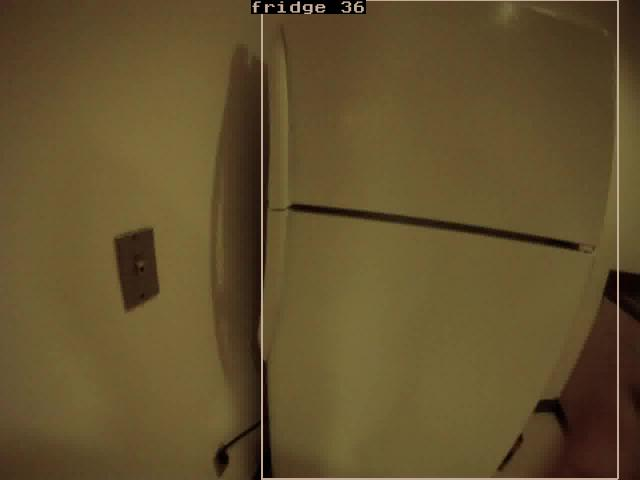
\includegraphics[width=2.0cm]{figures/fridge_passive.jpg}}}}
\subfigure[passive soap]{\bmvaHangBox{\fbox{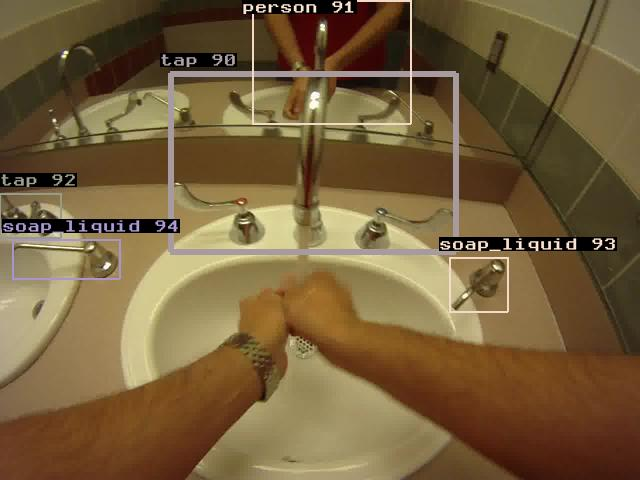
\includegraphics[width=2.0cm]{figures/soap_passive.jpg}}}}
\subfigure[passive mug]{\bmvaHangBox{\fbox{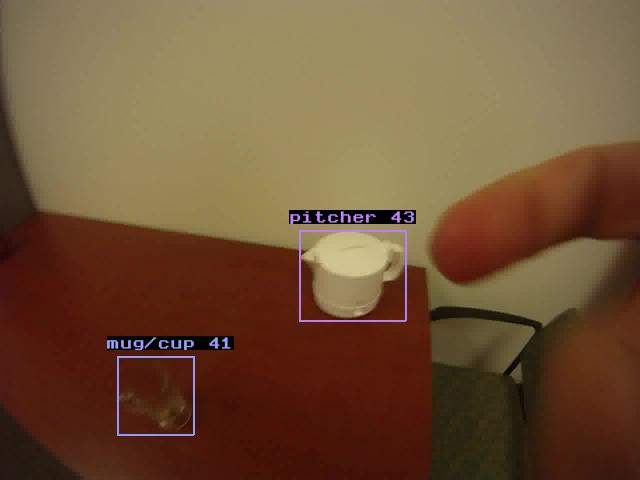
\includegraphics[width=2.0cm]{figures/mug_passive.jpg}}}}
\subfigure[passive micro]{\bmvaHangBox{\fbox{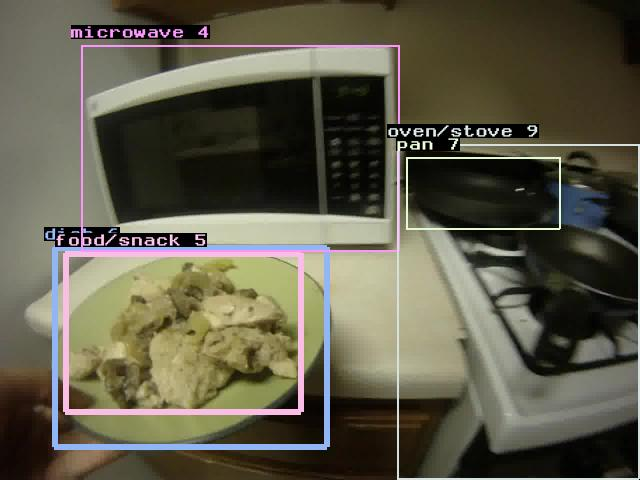
\includegraphics[width=2.0cm]{figures/micro_passive.jpg}}}}\\
\subfigure[active frig]{\bmvaHangBox{\fbox{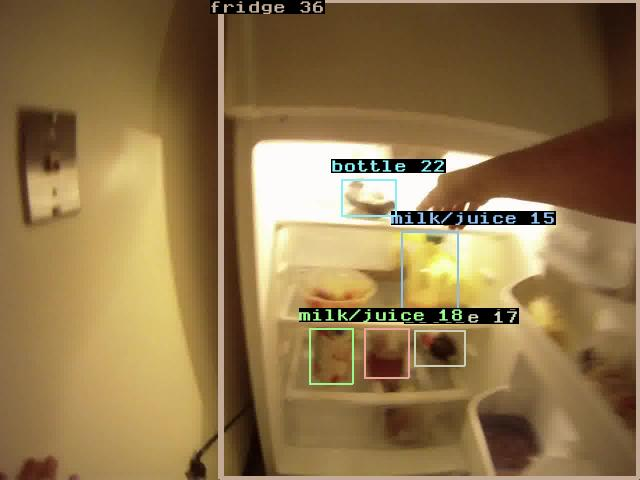
\includegraphics[width=2.0cm]{figures/fridge_active.jpg}}}}
\subfigure[active soap]{\bmvaHangBox{\fbox{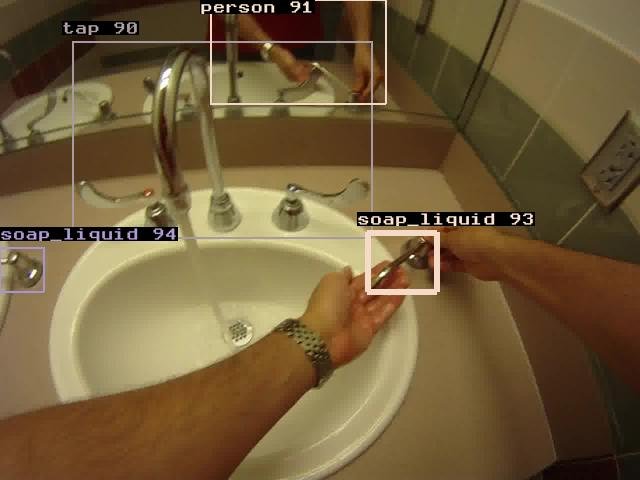
\includegraphics[width=2.0cm]{figures/soap_active.jpg}}}}
\subfigure[active mug]{\bmvaHangBox{\fbox{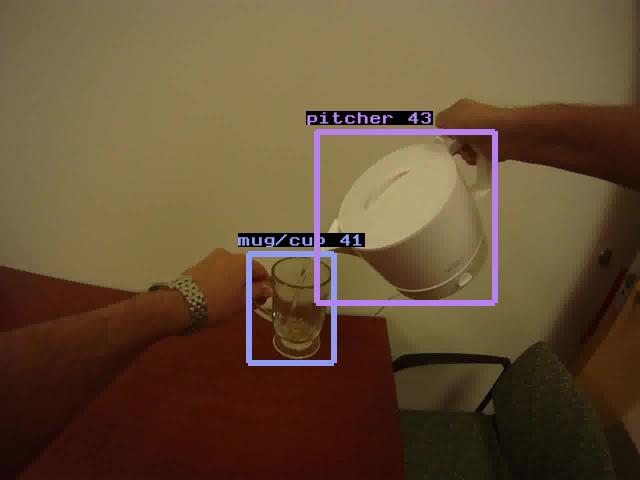
\includegraphics[width=2.0cm]{figures/mug_active.jpg}}}}
\subfigure[active micro]{\bmvaHangBox{\fbox{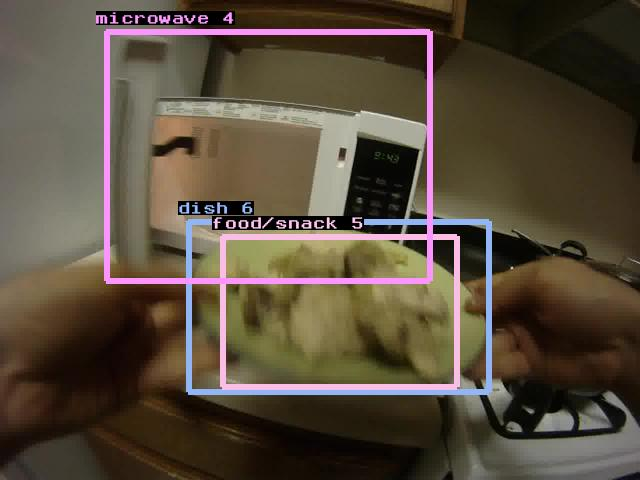
\includegraphics[width=2.0cm]{figures/micro_active.jpg}}}}
\end{tabular}
		   \caption{Example passive and active instances of four objects in ADL~\cite{Ramanan12}.}\vspace*{-0.2in}
\label{fig:active}
  \end{center}
 \end{figure}

 \vspace*{-0.05in}
\subsection{Detecting Active and Passive Objects}

Our goal is to robustly predict what type of activity is occurring in an egocentric video clip.  In contrast to traditional third-person video, egocentric actions are inherently defined by the objects the user is interacting with. Therefore, our representation is built on the pattern of objects that appear in space and time.  Specifically, the space-time pyramids we learn will count the frequency with which each object category appears in particular space-time regions.

Following~\cite{Ramanan12}, we make a distinction between active and passive instances of a given object category.  As noted in~\cite{Ramanan12}, objects' appearance can often change dramatically when the object is being interacted with.  For example, the refrigerator looks quite different when one passes by it closed, versus when one opens the door to grab some food.  Therefore, we train different deformable part model~\cite{DPM} detectors for active and passive versions of various objects of interest.\footnote{We use the public code and detection outputs provided by~\cite{Ramanan12}.}  Figure~\ref{fig:active} depicts example frames extracted from
the Activities of Daily Living (ADL)~\cite{Ramanan12} video sequences that show the visual differences between passive and
  active versions of four example objects.  In contrast to prior work, we exploit the active/passive object distinction to provide a helpful bias regarding where space-time partitions ought to be sampled, as we describe in the next section.
  
Once all object detectors have been applied to all frames in the training or test video, we have an $(x,y,t)$ coordinate for the bounding box center of each detected object.  Associated with each coordinate is its (predicted) object class (frig, microwave, etc.)


\subsection{Sampling Randomized Object-Centric Space-Time Pyramids}

Once we have the predicted object locations in all training videos, we are ready to construct space-time histogram pyramids.  A space-time pyramid will consist of multiple levels of bins, from coarse to fine.  For each bin, we record how many times each object class appears in its respective region of the video.  Then we concatenate these histograms over all pyramid levels to get a single descriptor for the video.  Thus, for a pyramid with $T$ total bins and a bank of $D$ total object detectors, the dimensionality of the entire descriptor will be $TD$.  Whereas past work uses a pyramid with uniformly placed bins~\cite{Choi08,Ramanan12}, we propose to generate randomized pyramids and then learn their most discriminative combination.

First we describe how to generate the randomized space-time pyramids (RSTP) \emph{without} the object-centric bias.  We consider each dimension $(x,y,t)$ in turn in a round-robin fashion to generate a cut (i.e., place a bin boundary).  Each cut is axis-aligned, meaning we use random shifts, but no random rotations.  We normalize all dimensions of an input video to length 1.  Then we sample a number uniformly at random in $[0,1]$, and use it to place the randomized cut in the current dimension.  Note that as we work our way recursively down the resulting tree, each subsequent cut is appropriately constrained by the span of its parent bin.  Level 0 of the pyramid is the entire video clip volume; level $i$ consists of all $8^i$ bins of depth $i$.

While boosting gives an automated way to select informative pyramids, its training time depends linearly on the number of candidates we include in the pool.  With so many possible randomized pyramids, the search space is extremely large.  Thus, intuitively, we can expect to pay a very high training cost to evaluate sufficiently many randomized pyramids to get good results.  

To avoid an excessive search, we focus the candidate pool in a way that is meaningful for egocentric data.  Rather than sample cuts uniformly at random, our idea is to sample the cuts according to the distribution of active objects as they appear in the training videos.  We refer to these as \emph{object-centric cuts} (OCC).  Specifically, we construct the empirical distribution of all active object occurrences, per dimension.  Then, when selecting each randomized cut, we sample its position according that distribution.  In this way we get pyramids that emphasize video regions likely to characterize the interactions between the camera wearer and objects.  For each pyramid, after generating one OCC per dimension, we generate all subsequent child cuts using a uniform distribution.  We found this was more effective than using OCC's at all levels, likely because we risk overfitting once bins are quite small in volume.  Note that while the OCC's are biased by active objects only, we still count both active and passive objects in the resulting histograms.



\begin{figure}
  \begin{center}
\begin{tabular}{ccc}
\bmvaHangBox{\fbox{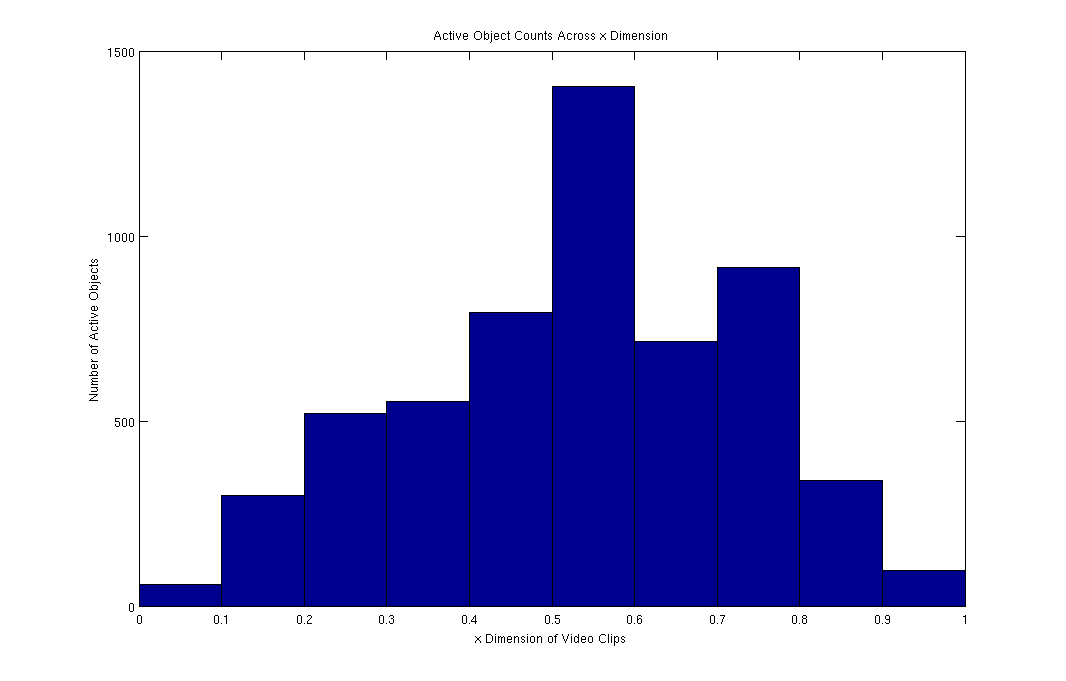
\includegraphics[width=3.5cm]{figures/active_obj_distr_x.png}}}&
\bmvaHangBox{\fbox{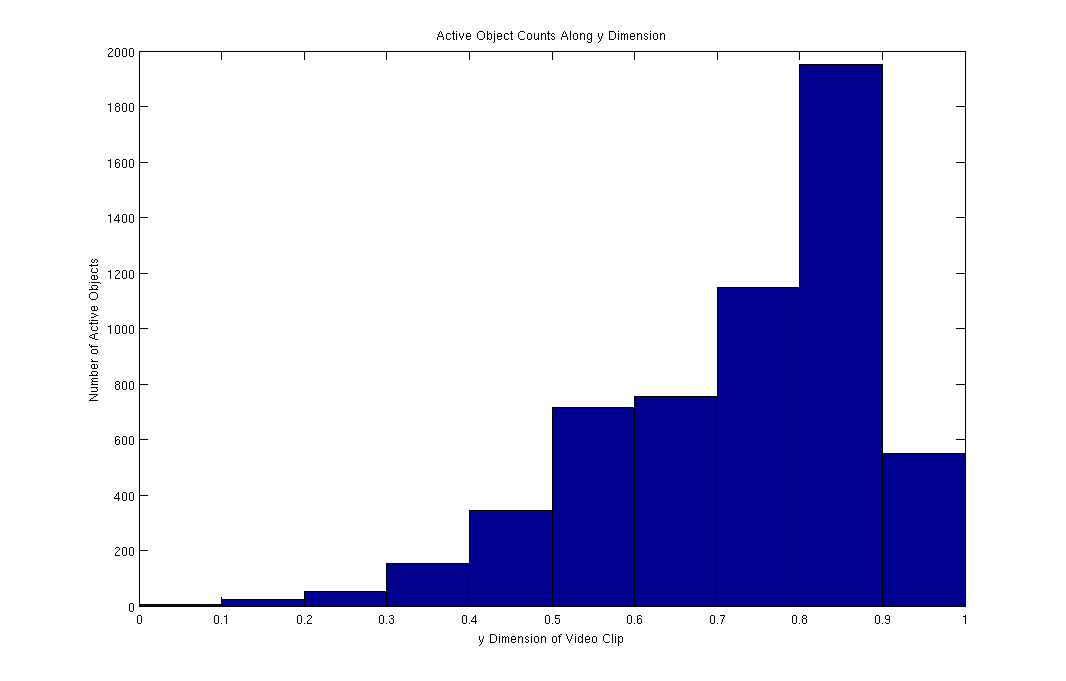
\includegraphics[width=3.5cm]{figures/active_obj_distr_y.png}}}
\bmvaHangBox{\fbox{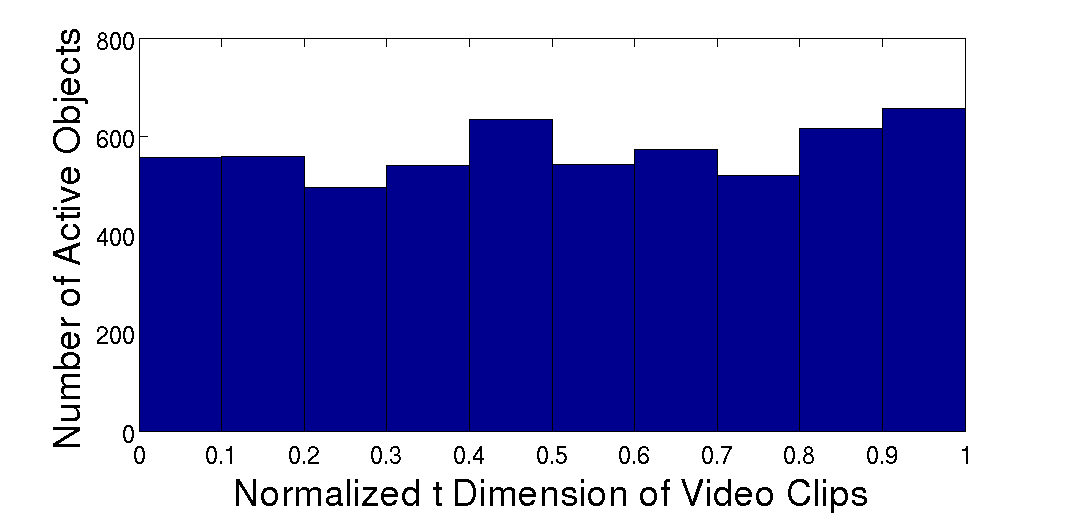
\includegraphics[width=3.5cm]{figures/active_obj_distr_t.png}}}
\end{tabular}
		   \caption{Histograms of detected active objects across $x$, $y$, and $t$ in the training data.}
\label{fig:histograms}
  \end{center}

\end{figure}


Figure~\ref{fig:histograms} shows the active object distributions for the ADL dataset we use to validate our approach.  We see that active objects tend to appear in the lower center field of view.  This conforms to our expectations, because active objects are close to the hands, which appear in the bottom portion of most frames from the chest mounted camera.  Furthermore, there is a slight bias favoring the right side of the field of view, likely because many camera wearers are right-handed.  Finally, we also observe that the distribution of active objects
  across the temporal dimension is nearly uniform; this reflects that we use object occurrences across all action types.  %%An alternative would be to generate action class-specific partitions.  Doing so might allow even more precise partitions, though will be more expensive for training.
  
  
%
%	\begin{figure}[t]
%		\begin{center}
%			%\fbox{\rule{0pt}{2in} \rule{0.9\linewidth}{0pt}}
%%			  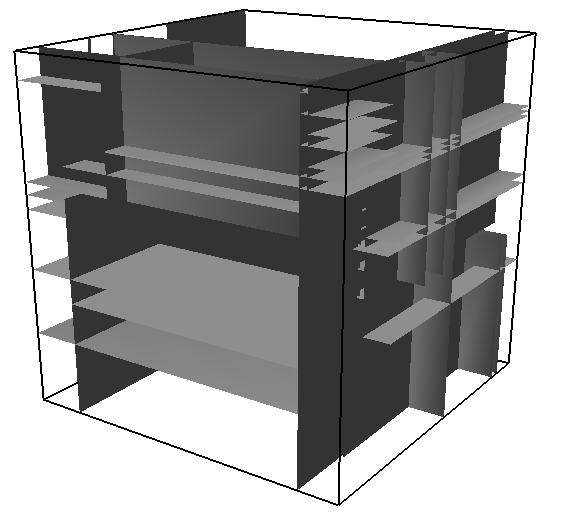
\includegraphics[width=6.0cm]{figures/lvl3-3.png}
% 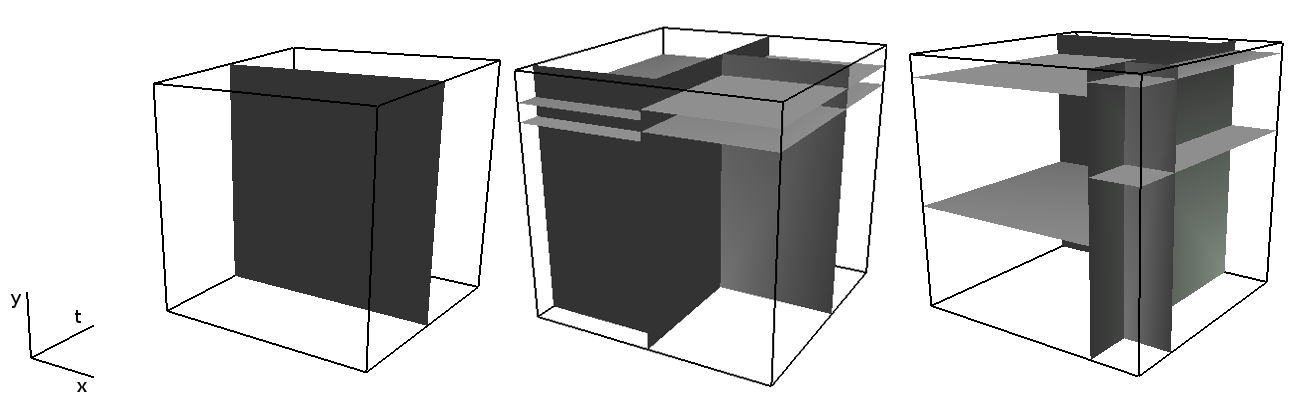
\includegraphics[width=6.0cm]{figures/allpyramids_axes.png}
%		\end{center}
%    \caption{temporal, unbiased, biased.  UPDATE An example 3-level object-centric partitioning scheme. Visible cuts along
%    the $y$ dimension correspond to locations known to frequently contain
%  active objects.}\label{fig:3types}
%	\end{figure}

Figure~\ref{fig:2dpartitions} shows some example frames with randomized shifts sampled using our object-centric strategy (a) or the simpler uniform strategy (b).  The object detections shown are from the ADL repository~\cite{Ramanan12}.  We see how OCC's successfully focus the histograms on regions in space-time where human-object interactions occur.  As a result, they may offer more discriminative cues that will be useful to the boosted classifier.

%
%  Figure 3 depicts an example 3-level object-centric partition scheme.
%  The salient feature to note is that visible splits along the $y$
%  dimension correspond to the observed distribution of active objects along
%  the $y$ dimension of the training data.
%




\begin{figure}[t]
  \begin{center}
  \begin{tabular}{c}
  \subfigure[Object-centric cuts]{
\begin{tabular}{ccccc}
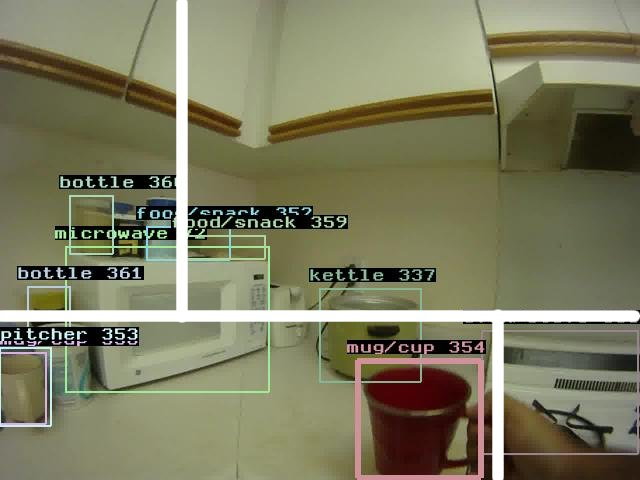
\includegraphics[width=2.2cm]{figures/ex1_biased.jpg}
%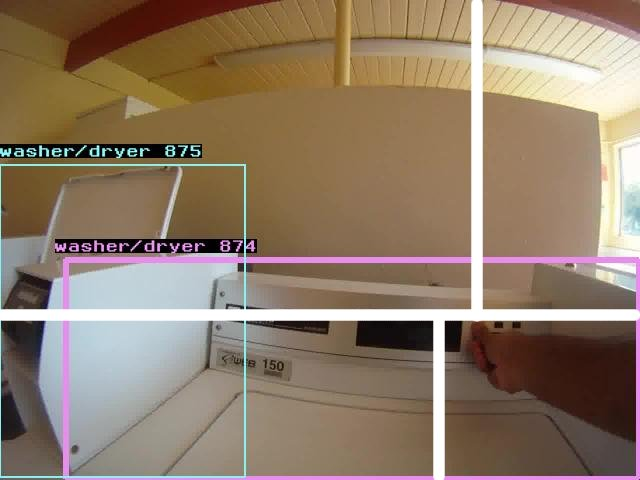
\includegraphics[width=2.2cm]{figures/ex2_biased.jpg}
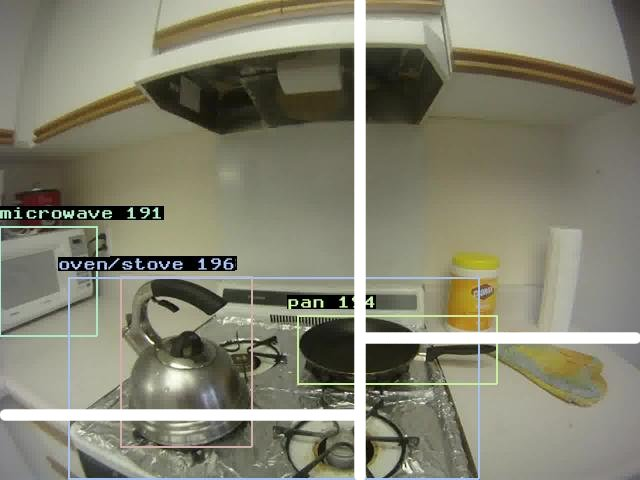
\includegraphics[width=2.2cm]{figures/ex3_biased.jpg}
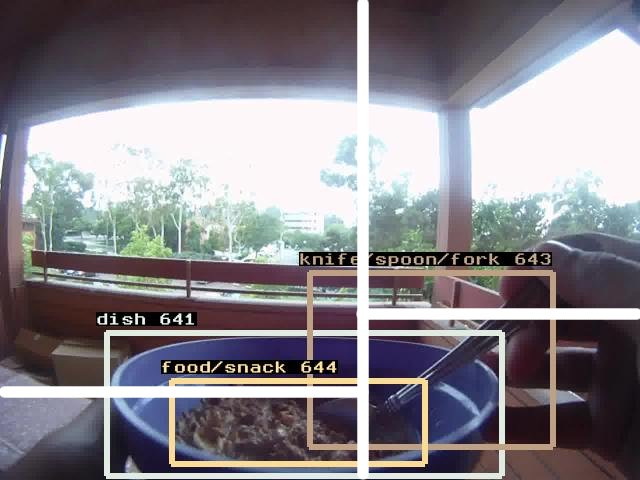
\includegraphics[width=2.2cm]{figures/ex4_biased.jpg}
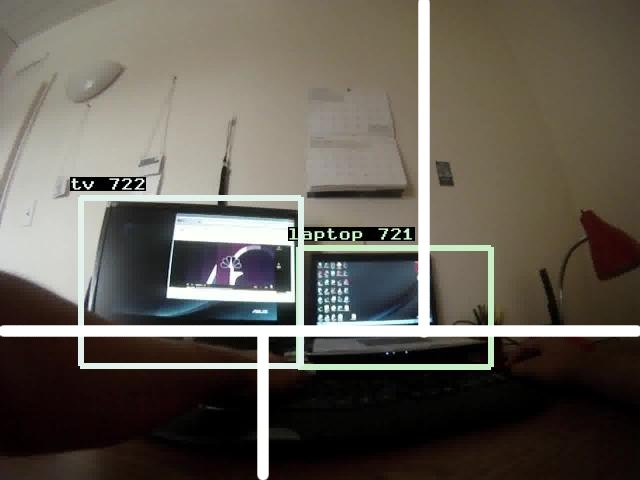
\includegraphics[width=2.2cm]{figures/ex5_biased.jpg}
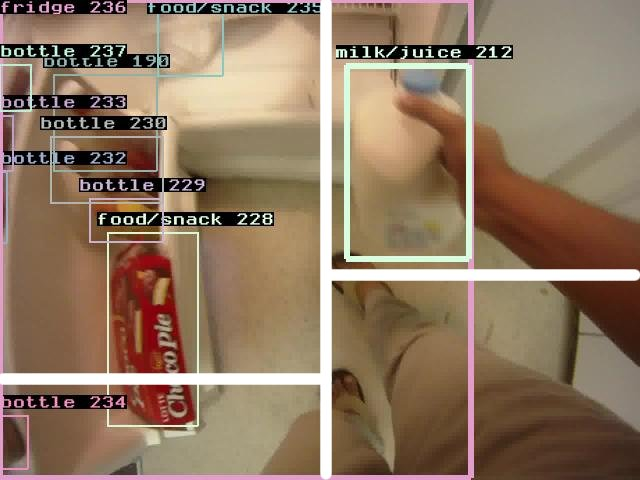
\includegraphics[width=2.2cm]{figures/ex6_biased.jpg}
\end{tabular}}\\
 \subfigure[Uniformly random shifts]{
\begin{tabular}{ccccc}
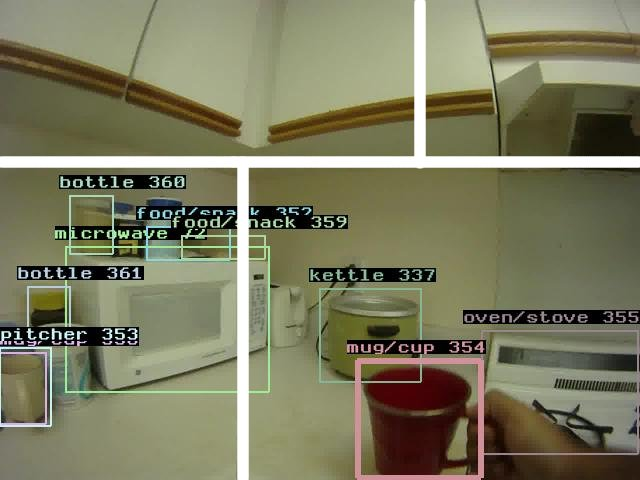
\includegraphics[width=2.2cm]{figures/ex1_unbiased.jpg}
%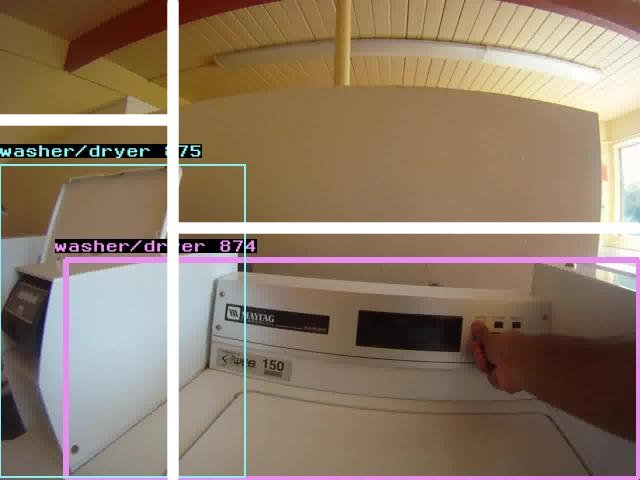
\includegraphics[width=2.2cm]{figures/ex2_unbiased.jpg}
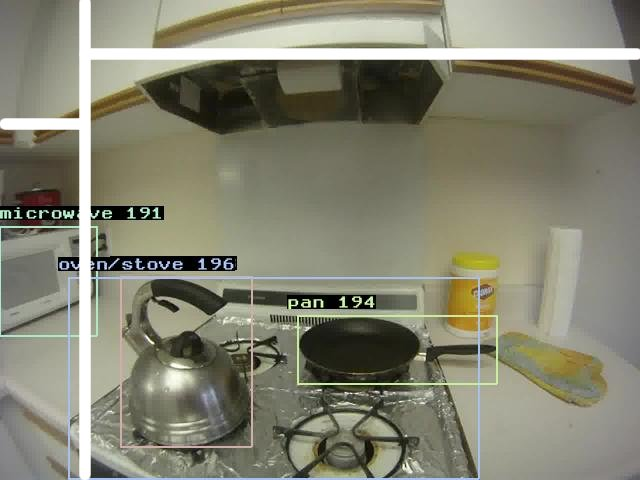
\includegraphics[width=2.2cm]{figures/ex3_unbiased.jpg}
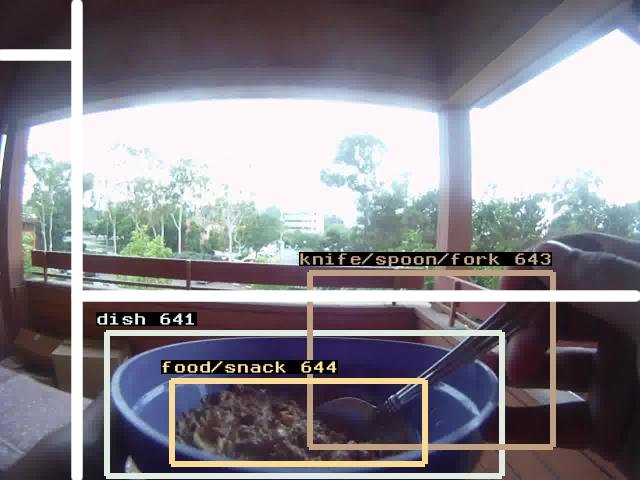
\includegraphics[width=2.2cm]{figures/ex4_unbiased.jpg}
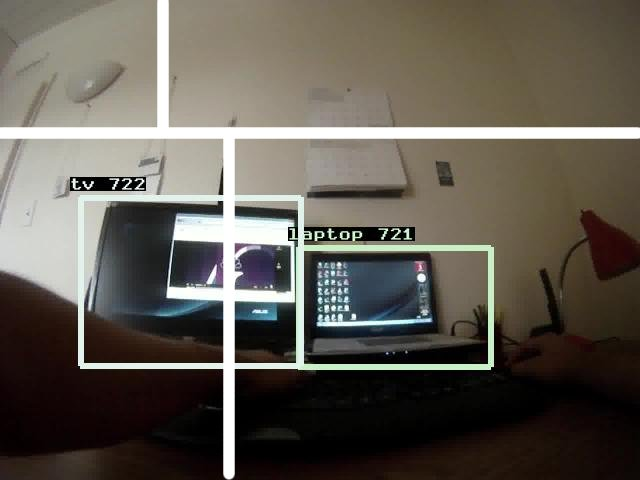
\includegraphics[width=2.2cm]{figures/ex5_unbiased.jpg}
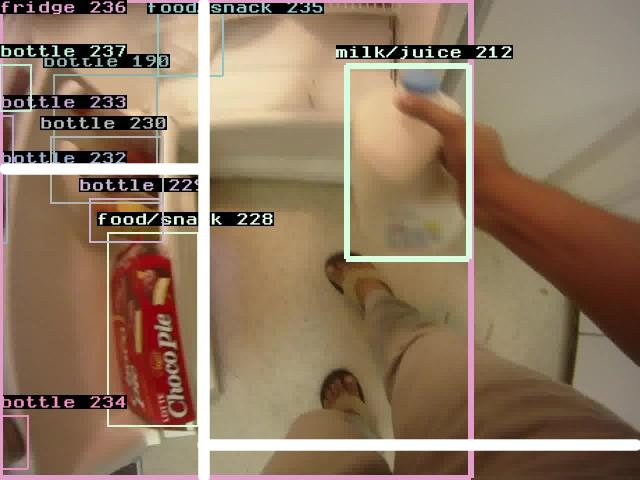
\includegraphics[width=2.2cm]{figures/ex6_unbiased.jpg}
\end{tabular}}
\end{tabular}
%\bmvaHangBox{\fbox{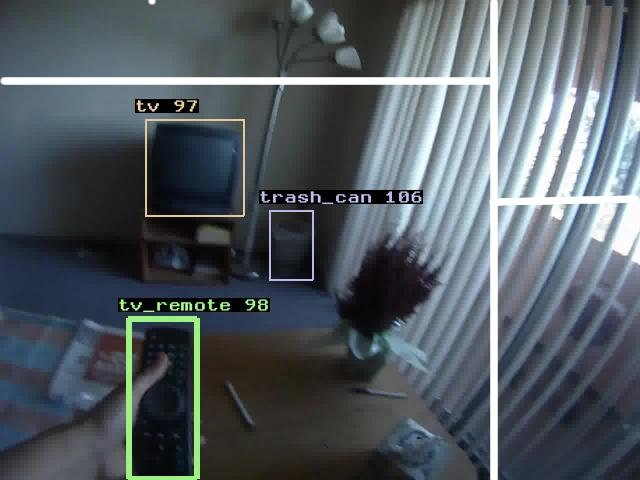
\includegraphics[width=5.9cm]{figures/unbiased_prt.jpg}}}&
%\bmvaHangBox{\fbox{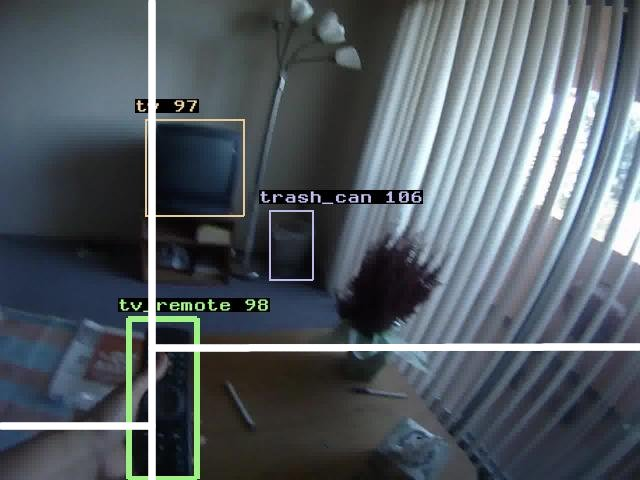
\includegraphics[width=5.9cm]{figures/biased_prt.jpg}}}\\
		   \caption{Example partitions using either object-centric (a) or uniformly sampled randomized cuts (b).  Note that for display purposes we show cuts on example 2D frames, but all cuts are 3D in space-time.  Using the proposed object-centric cuts, we better focus histograms surrounding the human-object interactions.}
\label{fig:2dpartitions}
  \end{center}
\end{figure}



\subsection{Boosting Discriminative Space-Time Pyramids}



\begin{figure}[t]
  \begin{center}
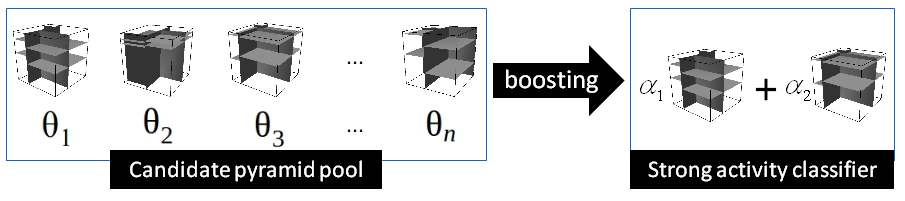
\includegraphics[width=9cm]{figures/concept-alg.png}
		   \caption{We take a pool of randomized space-time pyramids with object-centric cuts, and use boosting to select those that are most discriminative for egocentric activity recognition.}
\label{fig:concept-alg}
  \end{center}
\end{figure}


Finally, having constructed our object-centric pool of randomized pyramids, we are ready to apply boosting to select those that are most discriminative for the given activity recognition task (see Figure~\ref{fig:concept-alg}).  Boosting is a general learning algorithm in which one can combine a series of ``weak'' classifiers (better than chance) to form a single ``strong'' classifier.  In each round of boosting, the training examples are reweighted to emphasize training errors on those examples that were misclassified by weak classifiers selected in previous rounds. Here, our weak classifiers are non-linear (polynomial kernel) SVMs trained using one RSTP with OCC's.  We essentially use boosting to both select useful features (pyramids) and build the composite strong classifier.

For our implementation, we use the Stagewise Additive Modeling using a Multi-class Exponential loss function (SAMME) boosting approach of~\cite{Zhu06}, which naturally extends the original AdaBoost algorithm to the multi-class case without reducing it to multiple two-class problems.  We chose it due to its advantage of avoiding training individual classifiers for many one-vs.-rest (or one-vs.-one) problems and due to its ease of implementation.

SAMME boosting works as follows in our setting.  We take as input a collection of $N$ labeled training videos, where $(V_i, c_i)$ denotes a video clip and its associated ground-truth  activity label (drinking water, washing dishes, etc.).  We generate a pool of $M$ candidate RSTP's  $\{\theta_1, \theta_2, ..., \theta_M\}$, as described above.  For each RSTP $\theta$, we compute the corresponding histogram for each training example, using an object's bounding box center position $(x,y,t)$ to increment the appropriate bins.  We concatenate the histograms from all levels to create a single feature vector for each $V_i$ and each $\theta$.  Then we initialize a weight $w_i$ for each training example $V_i$ that is inversely proportional to the number of points with the same label as $V_i$. Giving larger weights to training examples of infrequently occurring actions helps to mitigate bias from imbalanced training data.

Next we train a separate weak multi-class SVM classifier (using the one-vs.one protocol in LIBSVM \cite{Chang11})
	 on the feature vectors resulting from representing the training
	data using each candidate partition pattern. 
 During each round of boosting we select the
	candidate partition $\theta_j$ that has the minimum  weighted training error.
  SAMME computes a weight for $\theta_j$ based on how many training
  examples were misclassified using $f_{\theta_j}$, the SVM classifier
  that was trained using the representation of the training data under
  $\theta_j$.
  At the end of each boosting iteration, we update the weights for each
  training example. Training examples that were previously misclassified are
  assigned higher weights to encourage correct classification in future
  boosting rounds.  Finally, we generate the
	final strong classifier $F$, which maximizes a weighted
  sum of correct classifications produced by each weak classifier.   Algorithm 1 summarizes these steps.
  
  Given a novel input video, we run the object detectors, then extract only those RSTP histograms that were selected by boosting, and apply $F$ to predict its activity label.
  
  %
%	\noindent\textbf{Algorithm 1:} Training via Multi-Class Boosting \\
%	\textbf{INPUT:}
%	\begin{itemize}
%		\item $N$ labeled training videos $\Phi = \{(V_i, c_i)\}_{i=1}^N$
%		\item A pool of $M$ partition patterns $\Theta = \{\theta\}$
%	\end{itemize}
%	\textbf{OUTPUT:}
%	\begin{itemize}
%		\item A strong video classifier $F$. For an unlabeled video $V$,
%			$c=F(V)$ is the predicted label for $V$.
%	\end{itemize}
%			\begin{enumerate}
%
%				\item For each $\theta \in \Theta$:
%					\begin{itemize}
%            \item Compute the representations of each $V_i \in \Phi$ using $\theta$
%						and train a multi-class classifier (SVM) $f_\theta$ on the
%            resulting feature vectors.
%					\end{itemize}
%
%				\item Initialize:
%					\begin{itemize}
%						\item A weight $w_i = \frac{1}{C N_{c_i}}$ for each video clip,
%							where $N_{c_i}$ is the number of videos with label $c_i$,
%              and $C$ is the number of distinct labels in the training data.
%						\item Current boosting round $j=0$.
%						%\item Current accuracy $\sigma_j = 0$.
%					\end{itemize}
%
%				\item For each round of boosting:
%					\begin{itemize}
%						\item Increment $j$.
%						\item Re-normalize the weight vector:
%              \begin{center}
%              $\forall i, w_i = \frac{w_i}{\Sigma_i^N w_i}$.
%              \end{center}
%					  \item For each pattern $\theta$,
%              compute its weighted classification error:
%              \begin{center}
%              $e_\theta = w \cdot \mbox{\textbf{I}}(f_\theta(V) \neq c)$
%              \end{center}
%						\item Choose the pattern $\theta_j$ with minimum weighted
%              classification error $e_j$.
%						\item Compute the weight for $\theta_j$:
%              \begin{center}
%              $\alpha_j = \mbox{log} \frac{1 - e_j}{e_j} + \mbox{log}(C-1)$
%              \end{center}
%						\item Update the weight vector:
%              \begin{center}
%							$w_i = w_i \cdot \mbox{exp}(\alpha_j \cdot
%							\mbox{\textbf{I}}(f_{\theta_j}(V_i) \neq c_i))$.
%              \end{center}
%						\item Generate the current strong classifier:
%              \begin{center}
%							$F(V) = \mbox{argmax}_c \Sigma_{m=1}^j \alpha_m \cdot
%							\mbox{\textbf{I}}(f_{\theta_m}(V) = c)$
%              \end{center}
%					\end{itemize}
%
%			\end{enumerate}
%	

  \footnotesize
  \hspace*{-0.19in}\line(1,0){365}\\
  \noindent\textbf{Algorithm 1:} Training a space-time pyramid classifier with boosting \\
  \line(1,0){365}\\
  \textbf{\scriptsize INPUT:}
  \begin{itemize}
    \item $N$ labeled training videos $\Phi = \{(V_i, c_i)\}_{i=1}^N$
    \item A pool of $M$ partition patterns $\Theta = \{\theta\}$
  \end{itemize}
  \textbf{\scriptsize OUTPUT:}
  \begin{itemize}
    \item A strong video classifier $F$. For an unlabeled video $V$,
      $c=F(V)$ is the predicted label for $V$.
  \end{itemize}
      \begin{enumerate}
        \item For each pattern $\theta \in \Theta$:
          \begin{itemize}
            \item Represent each $V_i \in \Phi$ using $\theta$
            and train an SVM classifier $f_\theta$ on the
            resulting feature vectors.
          \end{itemize}

        \item Initialize:
          \begin{itemize}
            \item A weight vector $w$ with $w_i = \frac{1}{C N_{c_i}}$ for each video
              where
              $N_{c_i}$ is the number of videos with label $c_i$, and
              $C$ is the number of distinct action labels.
            \item Current boosting round $j=0$.
          \end{itemize}

        \item For each round of boosting:
          \begin{itemize}
            \item Increment $j$ and re-normalize the weight vector $w$.
            \item For each pattern $\theta$,
              compute its weighted classification error:
              $\;\;\;\;e_\theta = w \cdot \mbox{\textbf{I}}(f_\theta(V) \neq c)$
            \item Choose the pattern $\theta_j$ with minimum weighted
              classification error $e_j$.
            \item Compute the weight for $\theta_j$ as:
              $\;\;\;\;\alpha_j = \mbox{log} \frac{1 - e_j}{e_j} + \mbox{log}(C-1)$
            \item Update the weight vector $w$:
              $\;\;\;\;\forall i: w_i = w_i \cdot \mbox{exp}(\alpha_j \cdot
              \mbox{\textbf{I}}(f_{\theta_j}(V_i) \neq c_i))$.
            \item Generate the current strong classifier as:
              $\;\;\;\;F(V) = \mbox{argmax}_c \Sigma_{m=1}^j \alpha_m \cdot
              \mbox{\textbf{I}}(f_{\theta_m}(V) = c)$
          \end{itemize}
      \end{enumerate}
  \line(1,0){365}\\
  \normalsize

  
  














%
%
%  \subsection{Complexity and Runtime}
%  The asymptotic complexity of training with $N$ training examples
%  and a pool of $M$ candidate partition schemes with $l$ levels using our
%  method is
%  \begin{center}
%  $O(N\cdot M \cdot 8^l \cdot t_{train} + b \cdot (N + M \cdot t_{test}))$
%  \end{center}
%  where $b$ denotes the number of boosting rounds, and $t_{train}$ and
%  $t_{test}$ denote the time to train and test a single SVM classifier on
%  $N$ feature vectors, respectively. Fortunately, $l$ remains small (never
%  exceeds 4 in our experiments). In order to predict the label for a single
%  test video clip $v$, we first need to compute representations of $v$ using
%  each partition scheme that was selected during boosting, then find the
%  class $c$ which maximizes a weighted sum of matching classifications using
%  each weak classifier selected during boosting.
%  Thus, the overall
%  asymptotic complexity of predicting the
%  label for a single video clip is
%  \begin{center}
%  $O(b \cdot 8^l + C \cdot b \cdot t)$
%  \end{center}
%  where $b$ is the number of boosting rounds, $C$ is the number of possible
%  activity labels, and $t$ is the time to predict the label of a test
%  example using a weak SVM classifier.
%

\vspace*{-0.2in}
\section{Results}

To validate our method, we use the Activities of Daily Living (ADL) dataset~\cite{Ramanan12}.  It is the largest available egocentric dataset for activity recognition, and to our knowledge, the most diverse and realistic.  It consists of hundreds of egocentric clips	(roughly 10 hours of video in total) collected from 20 people performing 18 actions in their own homes. These naturally
  occurring  actions are often related to hygiene or food preparation, e.g., combing hair, brushing teeth, doing laundry, washing dishes, etc. The authors also provide the object detector outputs from a part-based model~\cite{DPM} for 26 object classes, which we directly use as input to our method.  The objects include household items.  Five of the 26 detectors are for active versions of certain objects (namely, refrigerator, microwave, mug, oven/stove, and soap liquid).\footnote{The ADL dataset has been modified since the publication of
	\cite{Ramanan12}; because of this, running the published code gives
	slightly lower accuracy than the originally published numbers. We use the
  modified version of the dataset available from the authors webpage at the time of writing to
run all experiments.}  We use the authors' publicly available code to run their method for comparison.   
  
  
Throughout, we use five rounds of boosting and populate our candidate pool with 4-level pyramids.  Preliminary experiments showed that the finer-grained (4-level) pyramids were more often selected by boosting than their coarser 3-level counterparts, so we focus the pool accordingly for all results.  

  %
%  The work of \cite{Jiang12}, which uses a similar
%  pyramid-based boosting approach for 2D image recognition, found that using
%  pyramids with more than 3 levels actually led to a decrease in overall
%  accuracy due to over-segmentation of image space. However, we found that in the
%  3D case 4-level pyramids give better overall accuracy than coarser-grained
%  representations.

%  Object detectors are trained on videos from the
%  first 6 people and tested on the videos from the remaining 14 people.
%
%\begin{table}
%  \begin{center}
%\begin{tabular}{cc}
%\bmvaHangBox{\fbox{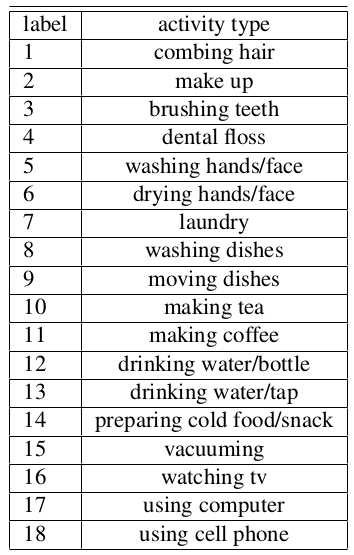
\includegraphics[width=4.0cm]{figures/actionlist.png}}}&
%\bmvaHangBox{\fbox{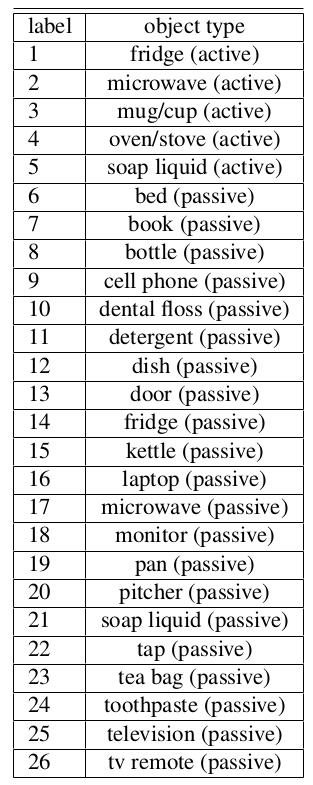
\includegraphics[width=4.0cm]{figures/objectlist.png}}}\\
%\end{tabular}
%		   \caption{Lists of action types and object types present in the
%       ADL dataset. Separate active and passive models are trained for fridge,
%     microwave, mug/cup, oven/stove, and soap liquid.}
%\label{fig:teaser}
%  \end{center}
% \end{table}


%
%	Each frame in the dataset
%	is annotated with activity labels and bounding boxes for detected objects and hand positions,
%	Additionally, each object is tagged as active or passive depending
%	on whether it is being interacted with.
%
%  One difficulty that can arise within egocentric
%  activity recognition is that activities can be temporarily interrupted by
%  other activities. For instance, while waiting for tea to brew a subject
%  may watch TV. For cases of such interruptions, to avoid unnecessary
%  complications resulting from frames being annotated with multiple
%  activities, the ADL dataset simply uses the label of the interrupting
%  action when a longer action is disrupted.


  We follow the exact evaluation protocol given in~\cite{Ramanan12}.  Specifically, we evaluate recognition accuracy using leave-one-person out: we test on videos from each person $i$ in turn, having trained on all remaining people.  We exclude the first 6 people, since their data was used to train the object detectors.
  
  
Table~\ref{table:results} shows the results, in terms of the average recognition rate over all 18 action classes.  We compare our boosted RSTP+OCC approach to four baselines.  The first baseline, bag-of-words (BoW), uses space-time interest points and HoG/HoF visual words, and represents what is now a standard representation for third-person action recognition.  The second baseline uses a bag-of-objects.  The third baseline, the Temporal Pyramid, is the method proposed in~\cite{Ramanan12}, and represents the state of the art on this dataset.  The fourth baseline, RSTP, is just like the proposed approach only it lacks the object-centric cuts.

Our approach outperforms all four baselines and improves the state of the art.  Compared to BoW, we have the advantage of high-level object-based features.  While the Temporal Pyramid~\cite{Ramanan12} also has this benefit, it is weaker than our method due to its reliance on a hand-crafted pyramid structure.  Notably, the proposed object-centric cuts are essential for our strong recognition result.  Simply using  boosting with purely randomized partitions (RSTP) is noticeably weaker.  This supports our claim that it is useful to bias bins according to object interactions for egocentric data.


  \begin{table}
		\begin{center}
			\begin{tabular}{|l|c|c|c|c|c|}
				\hline
        BoW & Bag-of-objects & TempPyr~\cite{Ramanan12} & Boost-RSTP & Boost-RSTP+OCC (ours) \\
				\hline\hline
        16.5\% & 34.9\% & 36.9\% & 33.7\% & \textbf{38.7\%}\\
				\hline
			\end{tabular}
		\end{center}
		\caption{Overall classification accuracy on ADL. Our method improves the state of the art.}\label{table:results}
	\end{table}

%
%
%  \begin{figure}
%  \begin{center}
%  \bmvaHangBox{\fbox{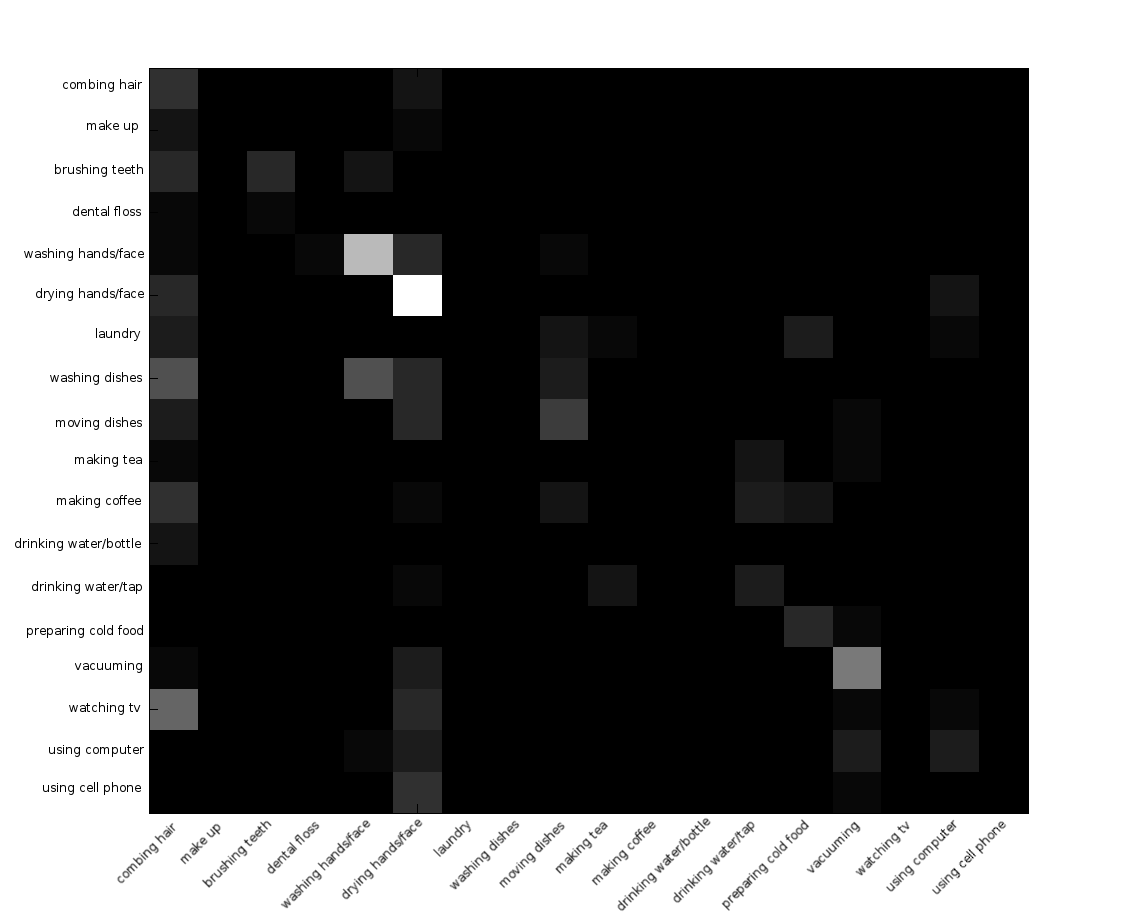
\includegraphics[width=6.0cm]{figures/confn2-labels.png}}}
%		   \caption{Confusion matrix for RSTP+OCC using detected active and
%       passive objects}
%  \label{fig:teaser}
%  \end{center}
%  \end{figure}



Looking more closely at our method's predictions, we find it has particularly good accuracy for ``combing hair'' and ``drying  hands/face''.  This suggests that the learned bins were able to usefully isolate the regular space-time relationships these actions exhibit.  On the other hand, we often confuse ``making tea'' and ``making coffee'', likely because they involve the same active objects.   Furthermore, since the distributions of objects across space-time are similar for both, and kettles and tea bags are not modelled as active objects, it is
  difficult for our boosting algorithm to select partitions that
  are discriminative for these classes. An extension of our method which
  allows selecting partitions on a per-class basis
  could allow for more fine-grained control and could help mitigate such
  issues, though would be more expensive.  We leave this as future work.


Compared to the Temporal Pyramid~\cite{Ramanan12}, we find out method is especially stronger for ``combing hair", ``brush teeth", ``dental floss".  This indicates that our learned spatial cuts are essential in scenes with similar objects appearing across different actions, as is the case with these bathroom-based activities.  For instance, while combing hair, floss or toothpaste might appear on the
counter, but floss or toothpaste would appear higher in the field of view when actually in use.







\begin{figure}
  \begin{center}
  \begin{tabular}{cc}
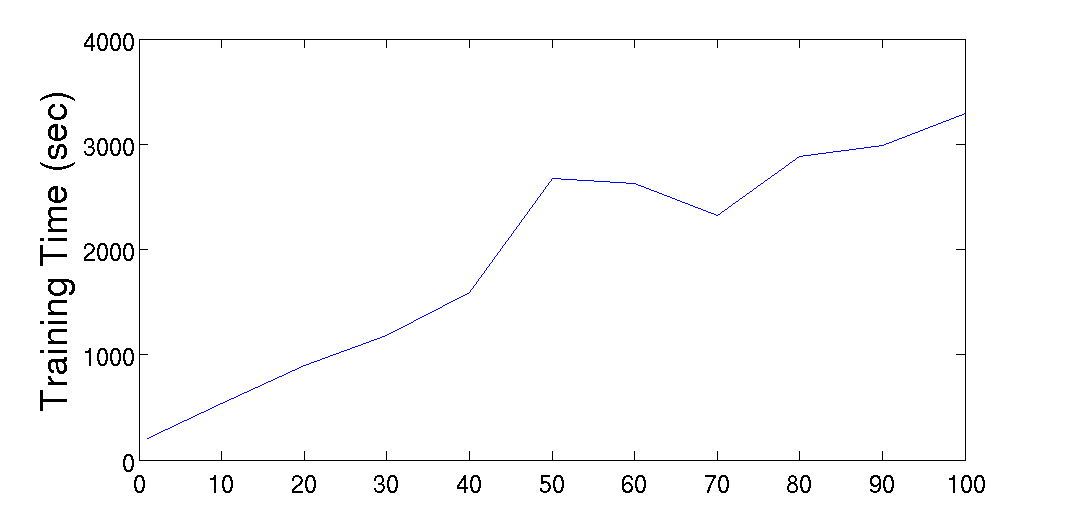
\includegraphics[width=5.2cm]{figures/runtime.png}
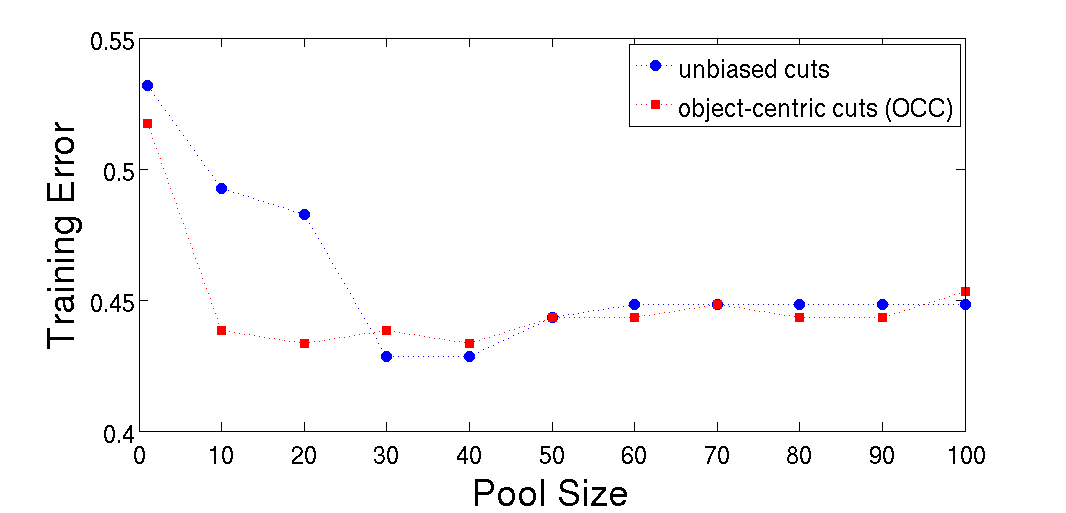
\includegraphics[width=5.2cm]{figures/trainerror.png}
\end{tabular}
		   \caption{Left: Training time as a function of pool size.  Right: Training error as function of pool size, for both uniformly sampled random shifts and the proposed object-centric partitions.  By focusing on object-centric shifts, we can achieve a stronger classifier with a smaller total pool, which improves training efficiency.}\vspace*{-0.1in}\label{fig:runtime-trainerror}
  \end{center}
\end{figure}

Figure~\ref{fig:runtime-trainerror} emphasizes the benefits of object-centric cuts.  On the left, we show the training time of running boosting with increasingly larger pools of candidate pyramids, averaged over five runs; run-time increases linearly with pool size.
On the right, we show the training error as a function of the pool size.  As desired, we see that the object-centric cuts lead to lower error with smaller pool sizes, compared to the unbiased RSTP's.  Essentially, our method focuses the pool on those candidates that \emph{a priori} have good chance at capturing discriminative aspects of the object distribution in space-time.  Thus, fewer total candidates must be explored to find good ones, and we can train the models with less total training time.

%  Larger improvements are visible with smaller pool sizes, and the difference
%  between the two pools diminishes as pool size increases. This conforms to
%  expectations because as the unbiased pool grows in size, it becomes more
%  likely to contain discriminative partition schemes, while the biased pool
%  is forced to contain discriminative partition schemes even at relatively
%  small pool sizes. This result suggests that by using object-centric
%  partitions rather than unbiased partitions, we can obtain good recognition
%  results even with a smaller pool, making our boosting algorithm less expensive
%  to compute.
%
%  \begin{figure}[t]
%		\begin{center}
%			%\fbox{\rule{0pt}{2in} \rule{0.9\linewidth}{0pt}}
%			  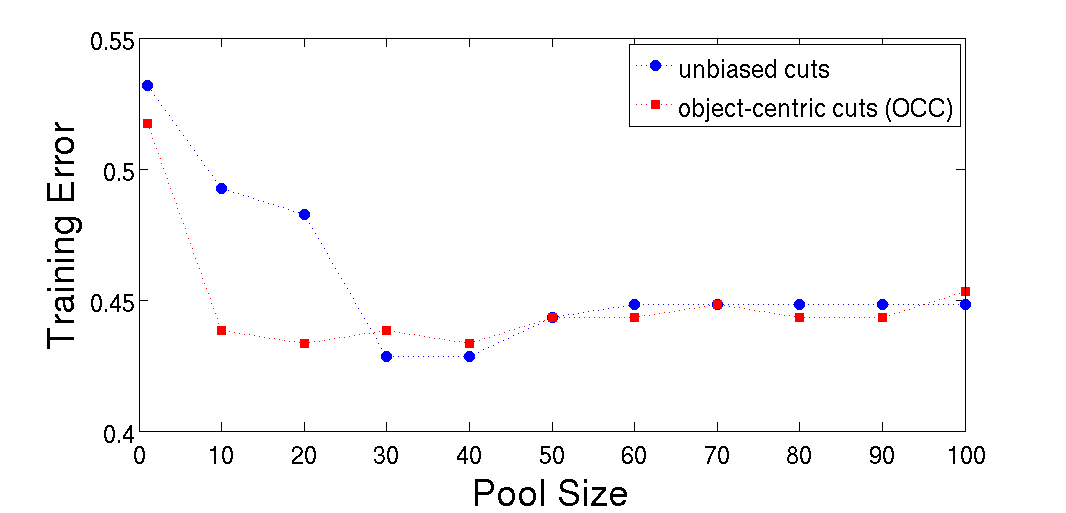
\includegraphics[width=1.0\linewidth]{figures/trainerror.png}
%		\end{center}
%		   \caption{Effect of using biased partition schemes. The object-centric
%         pool
%       usually has lower training error
%       than the pool of unbiased partition schemes. The most significant
%     improvement is visible at smaller pool sizes.}
%				\label{fig:long}
%				\label{fig:onecol}
%	\end{figure}
%
%	

\section{Conclusions and Future Work}

	Our main contribution is two-fold. We show how to learn the most
  discriminative partition schemes for spatio-temporal binning in action recognition, and
  we introduce object-centric cuts for egocentric data.  
  Our  approach improves on the current state of the art for recognizing activities of daily living from the first person viewpoint, and our
  experiments demonstrate the positive impact of taking active object
  locations into account via object-centric cuts.

  In future work, we intend to investigate ways of learning the most
  discriminative partition schemes on a per-class basis.
	Additionally, it may be possible to incorporate other related sampling biases. For example, our current strategy only implicitly accounts for the positions of hands via our OCC's, but it may be useful to incorporate explicit features about the hands.
	While we obtain good results using cuts that are
  planar and axis-aligned, one could easily extend the approach to populate the pool with non-linear cuts and/or randomized rotations. Such a method would
  make histogram computation more expensive, but may yield the discriminative
	partitions necessary for more fine-grained decisions.

  % egocentric analysis: recognition, summarization.
  % yong jae, lu zheng, fathi/ren (and some of their refs)
  % main point: importance of objects in egocentric vs other cues in other
  % domains
  Egocentric video is an increasingly popular topic in the computer vision
  community. Recent work has explored discovery of important people for
  automatic summarization of egocentric
  video \cite{Lee12}. The relationship between gaze and activity in an
  egocentric setting is explored in \cite{Fathi12}, which presents methods
  to predict activity given gaze, gaze given activity, and both activity and
  gaze given neither. Object recognition in an egocentric setting has been
  explored with promising results by \cite{Ramanan12, Fathi11, Ren09}.
  Activity recognition in an egocentric context has been investigated by
  \cite{Ramanan12, Fathi11_}.
  The main work related to our own is that carried out in \cite{Ramanan12}, 
  which introduces the ADL dataset we use to benchmark our method, 
  as well as detailed analysis of the the
	performance of several different classifiers. 
	
  Existing work has established that egocentric activities are object-driven
  in the sense that visible objects provide useful cues about what types of
  activities are occurring, rather than tracking of limb position or
  summarization of overall motion. In other words,
	egocentric activity recognition is ``all about
  the objects'' \cite{Ramanan12}, particularly the objects being interacted
  with (``active objects''), as
	recognition accuracy increases dramatically when locations of active
  objects in addition to passive objects are used as features. 




  % spatial binning strategies
  % kovashka, lazebnik, sharma, jiang (but not too much credit to jiang)
  Selection of binning strategies for features in a learned way has been throrougly explored in the
  spatial domain \cite{Sharma11, Jiang12} for image recognition, and some
  analysis of learning shapes of spatio-temporal regions on a per-class
  basis using low-level features has been conducted in the video domain \cite{Kovashka10}, but to
  our knowledge selection of binning strategies in a learned way has not
  been explored specifically in the egocentric domain.
  
	
  
	We use a version of the SAMME multi-class Ada-boost algorithm \cite{Zhu06}
  with randomized spatio-temporal pyramids to explore discriminative
  selection of partitions for video data, specifically in the egocentric
  domain.

\section{Approach}
  The goal of our algorithm is to robustly predict what type of activity is occurring in
  an egocentric video clip. In contrast to other forms of action
  recognition, egocentric action is ``object-driven'' in the sense that
  activities are well-defined by the objects the user is interacting with in
  a particular video sequence. Figure 1 depicts example frames extracted from
  video sequences that show the visual differences between passive and
  active versions of the same objects.
  
  Existing methods for non-egocentric activity
  recognition often use space-time interest points \cite{Laptev03} as features. In other
  words, in a non-egocentric setting action recognition is often driven by
  summarization of motion cues throughout video, while object locations can
  serve as effective features in an egocentric setting.

  Active objects, those which are being interacted with by the user in a
  given video clip, are especially helpful features for egocentric activity
  recognition \cite{Ramanan12}, yet there is little work in the literature
  exploring the best ways to pool video features across space-time. A common
  technique for pooling features is ``bag-of-words'', an orderless histogram
  of feature counts. This technique is simple, but does not encode any
  potentially useful relationships between features in space-time. The
  ``pyramid'' is an extension to bag-of-words that encodes space-time
  relationships between features by recursively
  subdividing an image or video into multiple subregions and concatenating
  bag-of-words histograms computed for each region. 

\begin{figure}
  \begin{center}
\begin{tabular}{cc}
\bmvaHangBox{\fbox{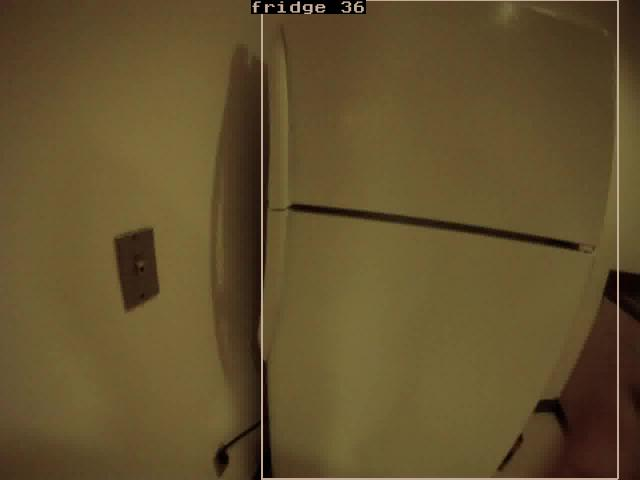
\includegraphics[width=4.0cm]{figures/fridge_passive.jpg}}}&
\bmvaHangBox{\fbox{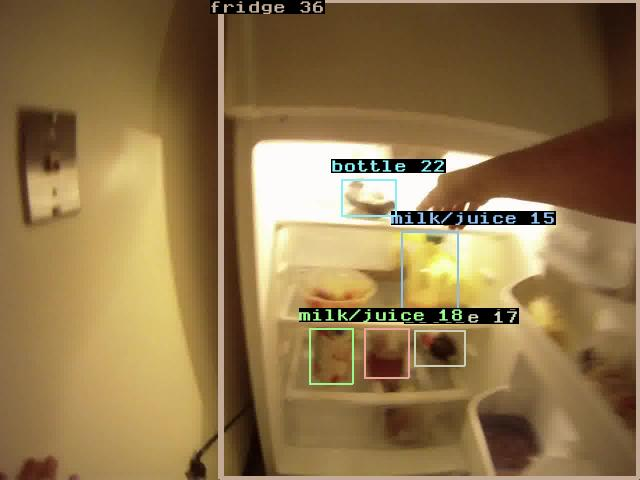
\includegraphics[width=4.0cm]{figures/fridge_active.jpg}}}\\
\bmvaHangBox{\fbox{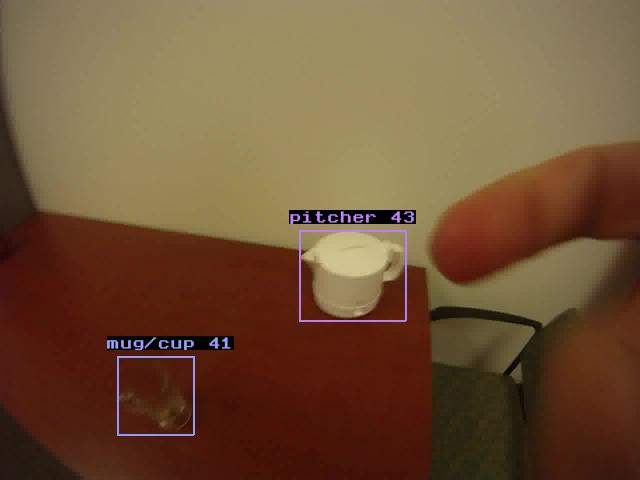
\includegraphics[width=4.0cm]{figures/mug_passive.jpg}}}&
\bmvaHangBox{\fbox{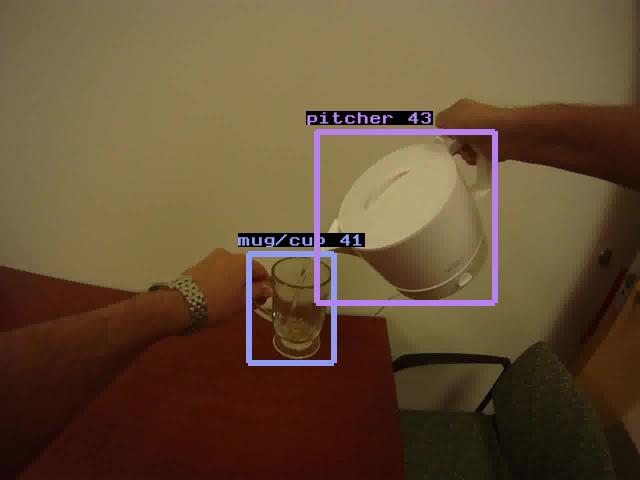
\includegraphics[width=4.0cm]{figures/mug_active.jpg}}}\\
\bmvaHangBox{\fbox{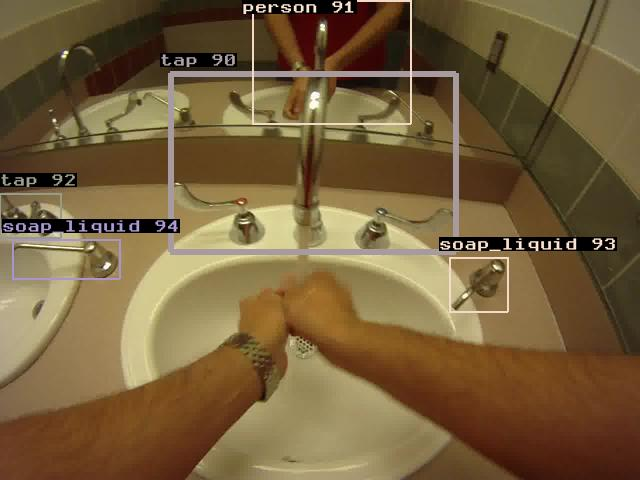
\includegraphics[width=4.0cm]{figures/soap_passive.jpg}}}&
\bmvaHangBox{\fbox{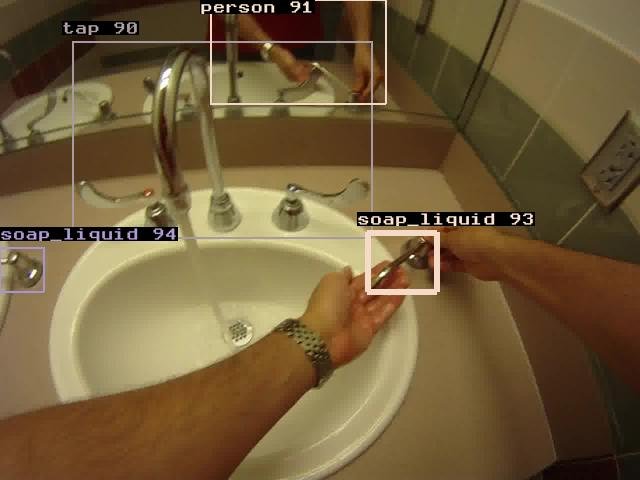
\includegraphics[width=4.0cm]{figures/soap_active.jpg}}}\\
\bmvaHangBox{\fbox{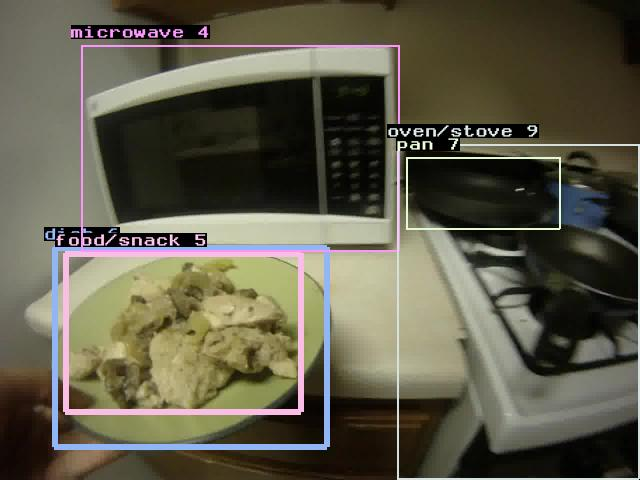
\includegraphics[width=4.0cm]{figures/micro_passive.jpg}}}&
\bmvaHangBox{\fbox{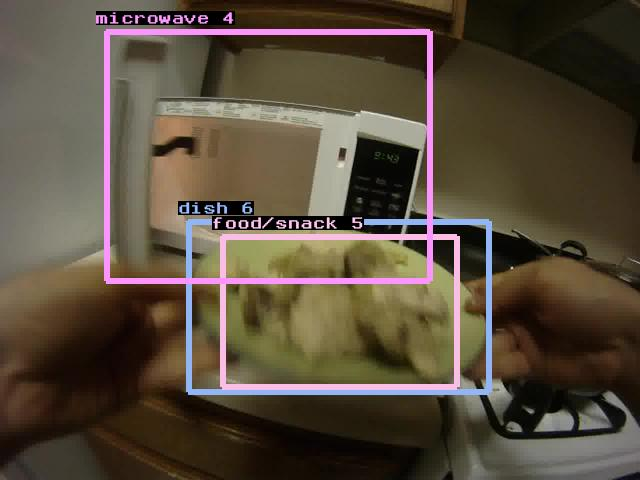
\includegraphics[width=4.0cm]{figures/micro_active.jpg}}}\\
\end{tabular}
		   \caption{Example frames extracted from the dataset. The left and
       right columns depict passive and active versions of the same objects,
     respectively.}
\label{fig:teaser}
  \end{center}
 \end{figure}
  Existing work relies on hand-coded partition schemes for computing
  pyramid representations of datapoints, which is a problematic approach
  because it is inflexible with respect to new data and can fail to capture
  the most meaningful relationships between features. To address this
  problem, we propose to randomly generate a pool of candidate partitioning
  schemes, then use a multi-class boosting algorithm to learn the most
  discriminative partition schemes and combine them into a final ``strong''
  classifier. 
  
  The intuition behind boosting is to train a set of classifiers and
  combine their output in such a way as to take advantage of the strengths
  of each individual classifier.
  This is accomplished by iteratively training classifiers on the training data.
  Datapoints are re-weighted after each iteration so that classifiers added during
  subsequent iterations tend to focus on examples that were previously
  misclassified.

	Our algorithm takes as input a collection of $N$ labeled training videos 
  where $(V_i, c_i)$ denotes a video clip and its associated ground-truth
  activity label,
	and a pool of $M$ candidate partition patterns 
  $\{\theta_1, \theta_2, ..., \theta_M\}$.
  We use the output of the
  aforementioned object detectors trained on composite object models as our features to be
  pooled. To convert from object bounding boxes to $(x,y,t)$ coordinates, we
  simply take the center of each bounding box.
  Thus, each training example $V_i$ is a set of $(o,x,y,t)$ object
  locations, where $o$ denotes an object label.

  To represent a particular training example $V_i$ using a particular
  partition scheme $\theta$, we compute separate bag-of-words histograms for
  each level in $\theta$, and concatenate all such histograms to form a
  final feature vector used in training.
  We initialize a weight
  $w_i$ for each
	training example $V_i$ that is inversely proportional to the number of points
	with the same class as $V_i$. Giving larger weights to training examples of
  infrequently occurring actions helps to mitigate any bias resulting from imbalanced
  training data.
  
  We train a separate ``weak''
  multi-class SVM 
  (using LIBSVM \cite{Chang11})
	classifier on the feature vectors resulting from representing the training
	data using each candidate partition pattern $\theta$.   During each round of boosting we select the
	candidate partition $\theta_j$ that is most discriminative (has minimum
  weighted training
	error, which is computed as the dot product between the weight vector $w$
  and an indicator of incorrect classifications using $f_\theta$).
  Next, we compute a weight for $\theta_j$ based on how many training
  examples were misclassified using $f_{\theta_j}$, the classifier
  that was trained using the representation of the training data under
  $\theta_j$.
  At the end of each boosting iteration, we update the weights for each
  training example. Training examples that were previously misclassified are
  assigned higher weights to encourage correct classification in future
  boosting rounds.
  Finally, we generate the 
	final strong classifier $F$, which maximizes a weighted
  sum of correct classifications produced by each weak classifier.\\
  \footnotesize
  \line(1,0){365}\\
	\noindent\textbf{Algorithm 1:} Training RSTP Classifier via Multi-Class Boosting \\
  \line(1,0){365}\\
	\textbf{\scriptsize INPUT:} 
	\begin{itemize}
		\item $N$ labeled training videos $\Phi = \{(V_i, c_i)\}_{i=1}^N$
		\item A pool of $M$ partition patterns $\Theta = \{\theta\}$
	\end{itemize}
	\textbf{\scriptsize OUTPUT:}
	\begin{itemize}
		\item A strong video classifier $F$. For an unlabeled video $V$, 
			$c=F(V)$ is the predicted label for $V$.
	\end{itemize}
			\begin{enumerate}
				\item For each pattern $\theta \in \Theta$:
					\begin{itemize}
            \item Represent each $V_i \in \Phi$ using $\theta$
						and train an SVM classifier $f_\theta$ on the
            resulting feature vectors.
					\end{itemize}

				\item Initialize:
					\begin{itemize}
						\item A weight vector $w$ with $w_i = \frac{1}{C N_{c_i}}$ for each video
              where 
				      $N_{c_i}$ is the number of videos with label $c_i$, and
              $C$ is the number of distinct action labels.
						\item Current boosting round $j=0$.
					\end{itemize}

				\item For each round of boosting:
					\begin{itemize}
						\item Increment $j$ and re-normalize the weight vector $w$.
					  \item For each pattern $\theta$,
              compute its weighted classification error:
              $\;\;\;\;e_\theta = w \cdot \mbox{\textbf{I}}(f_\theta(V) \neq c)$
						\item Choose the pattern $\theta_j$ with minimum weighted
              classification error $e_j$.
						\item Compute the weight for $\theta_j$ as:
              $\;\;\;\;\alpha_j = \mbox{log} \frac{1 - e_j}{e_j} + \mbox{log}(C-1)$
						\item Update the weight vector $w$:
							$\;\;\;\;\forall i: w_i = w_i \cdot \mbox{exp}(\alpha_j \cdot
							\mbox{\textbf{I}}(f_{\theta_j}(V_i) \neq c_i))$.
						\item Generate the current strong classifier as:
							$\;\;\;\;F(V) = \mbox{argmax}_c \Sigma_{m=1}^j \alpha_m \cdot
							\mbox{\textbf{I}}(f_{\theta_m}(V) = c)$
					\end{itemize}
			\end{enumerate}
  \line(1,0){365}\\
  \normalsize
  
  \subsection{Generating Randomized Spatio-Temporal Partitions (RSTP)}
  An RSTP is generated using a hierarchical partitioning of feature space.  
  We generate cuts independently in a round-robin manner over dimensions $(x, y, t)$. 
  Each cut is axis-aligned
  (we incorporate random shifts, but not random rotations).
  To construct a partition scheme that is easily applicable to videos of
  arbitrary size, we consider
  partitioning an ``idealized'' video clip that has all dimensions normalized
  to length 1. To generate a single cut we sample a random number from a
  uniform distribution subject to any constraints imposed by ``parent cuts'' and use
  this as a randomized offset for an appropriate axis-aligned plane. To
  construct an unbiased partition scheme we sample from a uniform
  distribution.
  
  To represent a video clip as a randomized spatio-temporal pyramid (RSTP)
  using a particular partition scheme we use the output of object detectors
  trained in \cite{Ramanan12}, which gives bounding boxes and object
  labels for each extracted frame. We use centroids of bounding boxes to
  obtain $(x,y,t)$ coordinates for each individual object.
  We compute histograms of detected
  objects for each individual level in the pyramid,
  where level 0 is the entire video clip volume and level $i$ is all the
  cells of depth $i$ in the pyramid. 
  Note that level $i$ has $8^i$ leaf
  cells. To form the final RSTP representation, we concatenate the
  histograms computed for each level to form a single feature vector.
  We can choose whether or not to include detected active objects when
  forming an RSTP representation of a video clip, however taking active
  objects into account gives a substantial improvement to overall
  classification accuracy. Figure 4(a) depicts a potential partitioning
  scheme that could arise when using uniform partition generation. In this
  case, the partition is not likely to be discriminative because all objects
  are located in a single region.
  
  \subsection{Generating Object-Centric Cuts (OCC)}
  There are many high-dimensional partition schemes that we could sample
  randomly, which suggests that a very large pool of candidate partition
  schemes is required to obtain good results. However, boosting is
  computationally expensive, so we would like to minimize the size of the
  pool while maintaining good results.
  One of the main contributions of our work is the ability to generate
  meaningfully biased randomized partition schemes that tend to be more discriminative
  than their unbiased counterparts.
  To accomplish this, we propose to replace the uniform distribution with a discrete
  approximation of the distribution of active objects across each dimension
  $(x, y, t)$
  and otherwise proceed normally.
  Figure 4(b) depicts a potential partitioning scheme that could arise when
  using object-centric partitioning. In this case, the example bin
  boundaries lie in a region containing an active object (tv remote), and
  the resulting partition scheme is likely to be more discriminative.

\begin{figure}
  \begin{center}
\begin{tabular}{cc}
\bmvaHangBox{\fbox{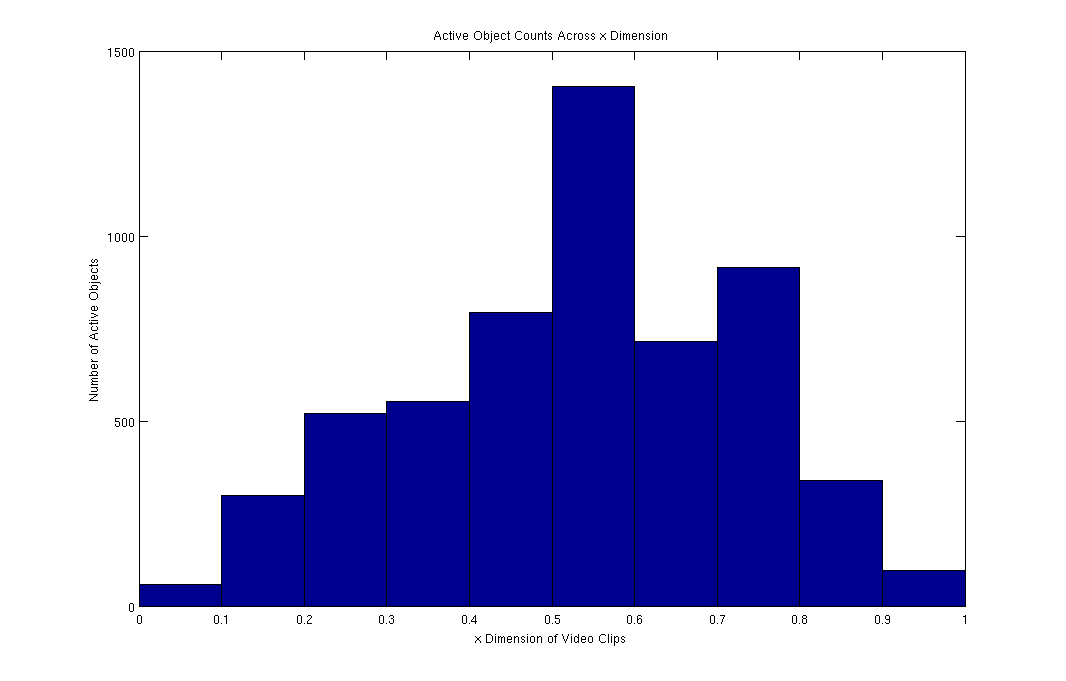
\includegraphics[width=5.9cm]{figures/active_obj_distr_x.png}}}&
\bmvaHangBox{\fbox{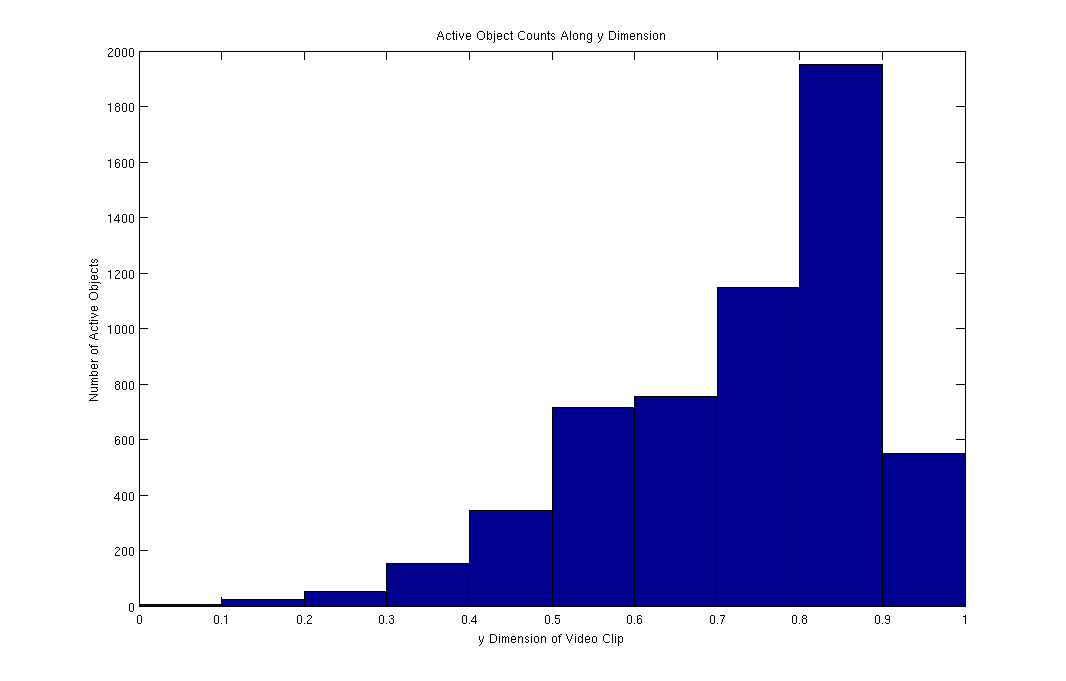
\includegraphics[width=5.9cm]{figures/active_obj_distr_y.png}}}\\
\end{tabular}
		   \caption{Histograms of detected active objects across the $x$ and
       $y$ spatial dimensions of training data. Active objects tend to appear in the lower
     center field of view. There is a slight bias favoring the
   right side of the field of view because many users are right-handed. }
\label{fig:teaser}
  \end{center}
\end{figure}
	
	From figure 2 we see that active objects often tend to occur in the lower center
	of the field of view. This conforms to our expectations, because
	the active objects are close to the hands which are in the lower field of
	view from an egocentric perspective. Active objects tend to occur on the
  right side of the field of view slightly more often because a large
  percentage of users are right-handed.
  The distribution of active objects
  across the temporal dimension is nearly uniform. 
  This distribution is computed across all action types; we do not compute
  separate active object distributions for each action class.
  Since different clips can have
  varying lengths with respect to time, we normalize the length of each
  video clip to 1 and consider relative temporal locations of active
  objects. 
	For biased partitions, we generate
  the first split along each dimension according to a distribution
  corresponding to the histograms of observed active object regions in the training data,
  and we generate all subsequent child cuts using a uniform distribution.
  For example, when generating a biased cut for the $y$ dimension, 
  we generate a random number between 0 and 1 that has a high probability of
  being in the range $(0.5, 0.9)$.
  We do not consider locations of passive objects at all during the
  generation of biased partition schemes.
  Since active objects are located
  in close spatial proximity to hands, creating object-centric partition schemes can
  be interpreted as implicitly taking into account information about hand
  locations.
	\begin{figure}[t]
		\begin{center}
			%\fbox{\rule{0pt}{2in} \rule{0.9\linewidth}{0pt}}
			  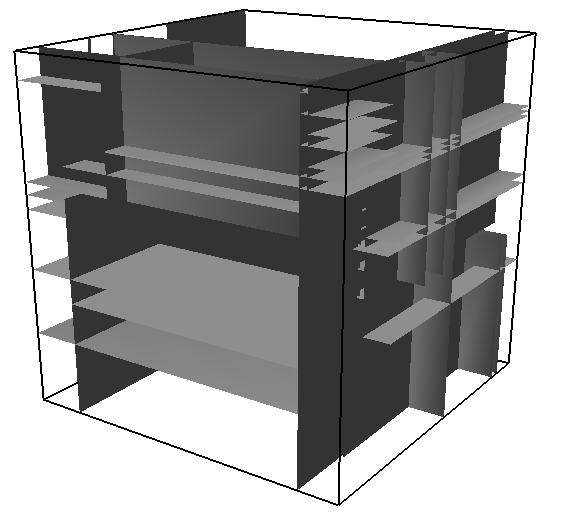
\includegraphics[width=6.0cm]{figures/lvl3-3.png}
		\end{center}
    \caption{An example 3-level object-centric partitioning scheme. Visible cuts along
    the $y$ dimension correspond to locations known to frequently contain
  active objects.} 
				\label{fig:long}
				\label{fig:onecol}
	\end{figure}
  
  Figure 3 depicts an example 3-level object-centric partition scheme. 
  The salient feature to note is that visible splits along the $y$
  dimension correspond to the observed distribution of active objects along
  the $y$ dimension of the training data.
  

\begin{figure}
  \begin{center}
\begin{tabular}{cc}
\bmvaHangBox{\fbox{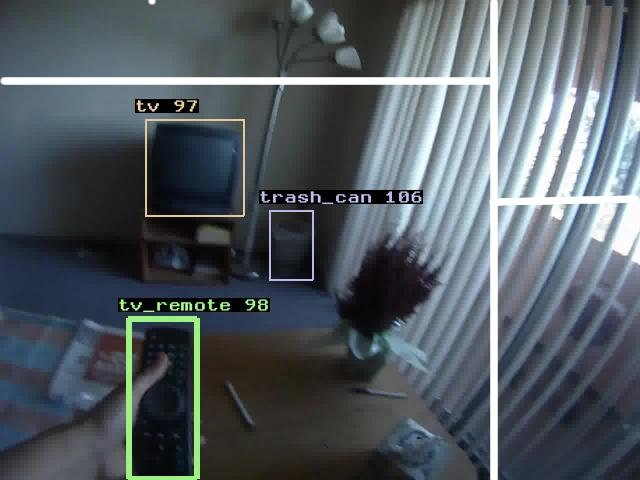
\includegraphics[width=5.9cm]{figures/unbiased_prt.jpg}}}&
\bmvaHangBox{\fbox{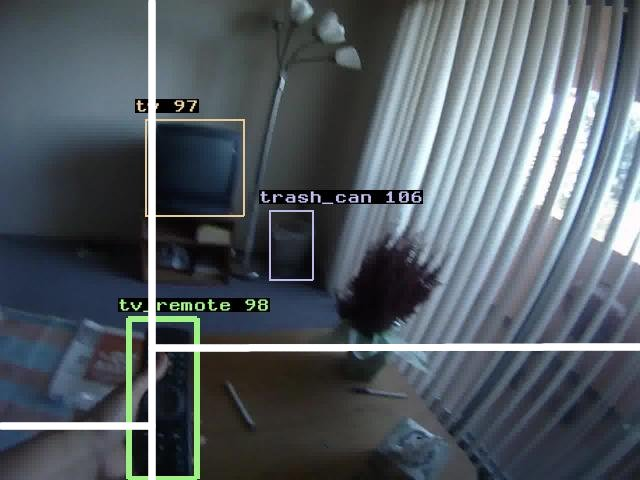
\includegraphics[width=5.9cm]{figures/biased_prt.jpg}}}\\
(a)&(b)\\
\end{tabular}
		   \caption{Potential partition schemes that could result using uniform
       (a) and object-centric (b) partition generation. The partition scheme
     resulting from using object-centric partition is likely to be more
   discriminative.}
\label{fig:teaser}
  \end{center}
\end{figure}
  
  \subsection{Complexity and Runtime}
  The asymptotic complexity of training with $N$ training examples 
  and a pool of $M$ candidate partition schemes with $l$ levels using our
  method is 
  \begin{center}
  $O(N\cdot M \cdot 8^l \cdot t_{train} + b \cdot (N + M \cdot t_{test}))$
  \end{center}
  where $b$ denotes the number of boosting rounds, and $t_{train}$ and
  $t_{test}$ denote the time to train and test a single SVM classifier on
  $N$ feature vectors, respectively. Fortunately, $l$ remains small (never
  exceeds 4 in our experiments). In order to predict the label for a single
  test video clip $v$, we first need to compute representations of $v$ using
  each partition scheme that was selected during boosting, then find the
  class $c$ which maximizes a weighted sum of matching classifications using
  each weak classifier selected during boosting.
  Thus, the overall
  asymptotic complexity of predicting the
  label for a single video clip is 
  \begin{center}
  $O(b \cdot 8^l + C \cdot b \cdot t)$
  \end{center}
  where $b$ is the number of boosting rounds, $C$ is the number of possible
  activity labels, and $t$ is the time to predict the label of a test
  example using a weak SVM classifier.
  
\begin{figure}
  \begin{center}
\bmvaHangBox{\fbox{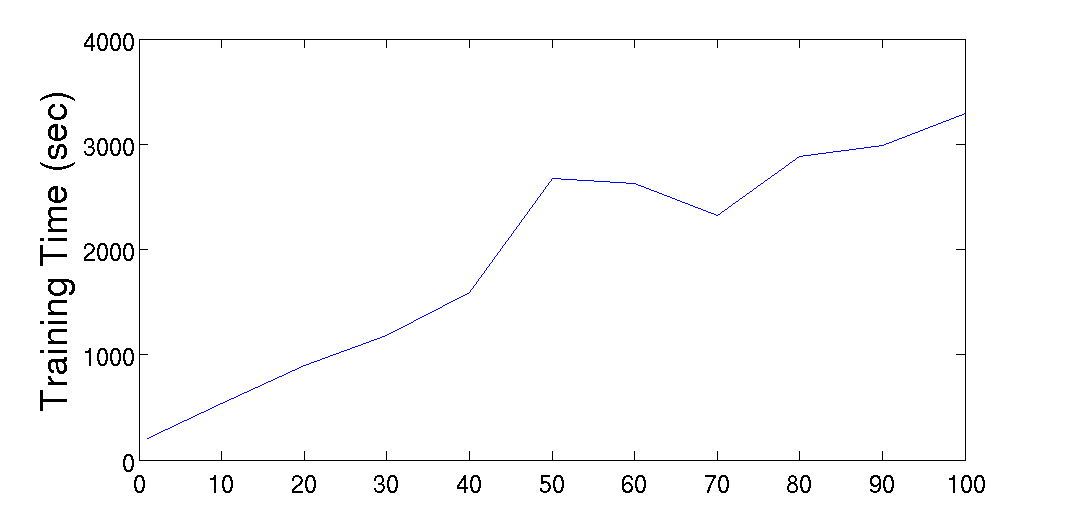
\includegraphics[width=9.0cm]{figures/runtime.png}}}\\
		   \caption{Running times for our method as a function of pool size.}
\label{fig:teaser}
  \end{center}
\end{figure}
  Figure 5 depicts empirically determined running times for our method on a
  single ``fold'' of the cross-validation experiment described in section
  3.1. For each pool size we present mean execution time across 5 separate
  executions. Running time is linear with respect to pool size.
  

\section{Results}
  In this section we briefly describe properties of the dataset we use to
  benchmark our method and present results from experiments we conducted. We
  evaluate our overall recognition accuracy and show that it improves the
  current state of the art, and we demonstrate the superior discriminative
  power of object-centric partition schemes.

  The ADL dataset consists of hundreds of egocentric video clips
	(roughly 10 hours of video in total) collected from 20 people performing
	18 types of unscripted actions in their own homes. These naturally
  occurring
  actions are often related to hygiene or food preparation and are more
  varied than actions presented in previous datasets such as that of \cite{Fathi11}.
  There are 26 different 
	types of detected objects, including 5 active and 21 passive objects. 
  Lists of activity types and object types are given in Table 1.
  Object detectors are trained on videos from the
  first 6 people and tested on the videos from the remaining 14 people.

\begin{table}
  \begin{center}
\begin{tabular}{cc}
\bmvaHangBox{\fbox{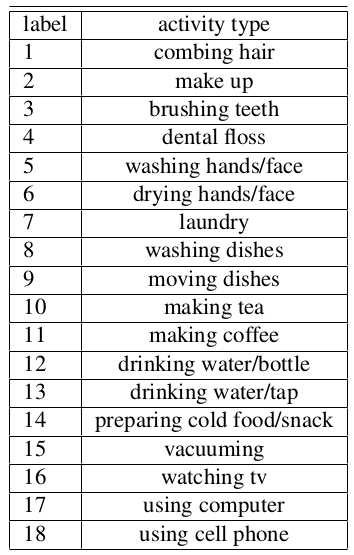
\includegraphics[width=4.0cm]{figures/actionlist.png}}}&
\bmvaHangBox{\fbox{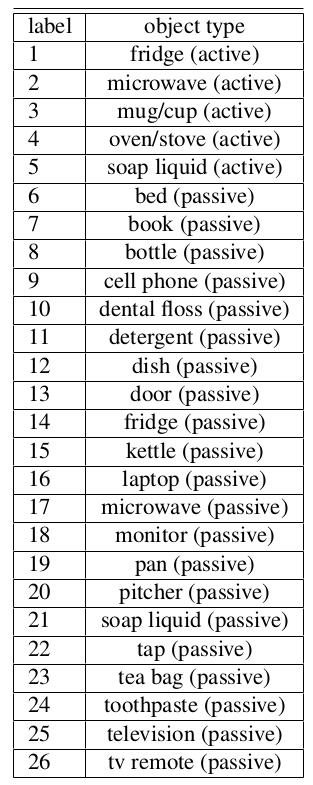
\includegraphics[width=4.0cm]{figures/objectlist.png}}}\\
\end{tabular}
		   \caption{Lists of action types and object types present in the
       ADL dataset. Separate active and passive models are trained for fridge,
     microwave, mug/cup, oven/stove, and soap liquid.}
\label{fig:teaser}
  \end{center}
 \end{table}
  

  
	Each frame in the dataset
	is annotated with activity labels and bounding boxes for detected objects and hand positions, 
	Additionally, each object is tagged as active or passive depending
	on whether it is being interacted with. 
  
  One difficulty that can arise within egocentric
  activity recognition is that activities can be temporarily interrupted by
  other activities. For instance, while waiting for tea to brew a subject
  may watch TV. For cases of such interruptions, to avoid unnecessary
  complications resulting from frames being annotated with multiple
  activities, the ADL dataset simply uses the label of the interrupting
  action when a longer action is disrupted.
  

	The ADL dataset has been modified since the publication of
	\cite{Ramanan12}; because of this, running the published code gives
	slightly lower accuracy than the originally published numbers. We use the
  modified version of the dataset available from the authors webpage at the time of writing to
  benchmark our method.   \subsection{Action Recognition Performance}
  Following \cite{Ramanan12}, we evaluate recognition performance on the ADL
  dataset using a form of cross
	validation (the video clips from person $i$ are used as a held out validation set, and
	training occurs using the video clips from the remaining people).
  We exclude videos from the first 6 people
  (because they were used to train the object detectors) from our
  experiments.

	  Table 2 shows a comparison of overall classification accuracy between our
  approach and the method based on temporal pyramids which is
  presented in \cite{Ramanan12}. The temporal pyramid
  has two levels, formed by making a single cut along the temporal
  dimension and no cuts along the spatial dimensions.
  These results were obtained
  using both active (being interacted with) and passive detected objects.
  The consideration of active objects when constructing feature vectors
  gives a significant improvement over just including passive objects.

  \begin{table}
		\begin{center}
			\begin{tabular}{|l|c|c|c|c|c|}
				\hline
        BoW & Temporal Pyramid \cite{Ramanan12} & RSTP & RSTP+OCC \\
				\hline\hline
        34.9\% & 36.9\% & 33.7\% & 38.7\%\\
				\hline
			\end{tabular}
		\end{center}
		\caption{Overall classification accuracy on pre-segmented video clips,
    evaluated using a form of cross validation. Our boosted RSTP+OCC classifier
  improves on the current state of the art.}
	\end{table}
  
	For this experiment we tried pools of 4-level partitioning schemes of
  varying sizes with a varying number of boosting rounds. The numbers
  presented in Table 2 were obtained with 5 boosting rounds and a pool of
  size 70.
  The work of \cite{Jiang12}, which uses a similar
  pyramid-based boosting approach for 2D image recognition, found that using
  pyramids with more than 3 levels actually led to a decrease in overall
  accuracy due to over-segmentation of image space. However, we found that in the
  3D case 4-level pyramids give better overall accuracy than coarser-grained
  representations.


  
  \begin{figure}
  \begin{center}
  \bmvaHangBox{\fbox{\includegraphics[width=10.0cm]{figures/confn2-labels.png}}}
		   \caption{Confusion matrix for RSTP+OCC using detected active and
       passive objects}
  \label{fig:teaser}
  \end{center}
  \end{figure}
 	As seen in Figure 6, our method has particularly good
  performance for activity types 5 and 6 (``combing hair'' and ``drying
  hands/face'', respectively). Some activity types on which our method does
  poorly are 10 and 11, which are ``making tea'' and ``making coffee'',
  respectively (see Table 1 for a full listing of activity types present in
  the ADL dataset). Since the two activity types are similar in the sense that
  they involve the same active objects, it is not
  unexpected that a recognition system would confuse them often.
  Furthermore, since the distributions of objects across space-time are
  similar, and kettles and tea bags are not modelled in an active way, it is
  difficult for our boosting algorithm to select partitioning schemes that
  are discriminative for these classes. An extension of our method which
  allowed selection of discriminative partition schemes on a per-class basis
  could allow for more fine-grained control and could help mitigate such
  issues.




  

  % training error exp
  \subsection{Effect of Object-Centric Partition Schemes}
  To concretely illustrate the improvement obtained from using a
  object-centric partitions, we created separate pools containing 4-level
  partition schemes of each bias type and
  repeatedly ran our boosting algorithm, computing training error and adding additional
  partitions to each pool between runs. Results from this experiment are
  depicted in Figure 7. The pool containing object-centric partitions 
  usually had a lower training error than the unbiased pool.
  Larger improvements are visible with smaller pool sizes, and the difference
  between the two pools diminishes as pool size increases. This conforms to
  expectations because as the unbiased pool grows in size, it becomes more
  likely to contain discriminative partition schemes, while the biased pool
  is forced to contain discriminative partition schemes even at relatively
  small pool sizes. This result suggests that by using object-centric
  partitions rather than unbiased partitions, we can obtain good recognition
  results even with a smaller pool, making our boosting algorithm less expensive
  to compute.
 
  \begin{figure}[t]
		\begin{center}
			%\fbox{\rule{0pt}{2in} \rule{0.9\linewidth}{0pt}}
			  \includegraphics[width=1.0\linewidth]{figures/trainerror.png}
		\end{center}
		   \caption{Effect of using biased partition schemes. The object-centric
         pool
       usually has lower training error
       than the pool of unbiased partition schemes. The most significant
     improvement is visible at smaller pool sizes.}
				\label{fig:long}
				\label{fig:onecol}
	\end{figure}
	
\bibliography{egbib}
\end{document}
